\title{计算机图形学}
\author{李宇轩}

\documentclass{xNoteBook}

\usepackage{xCommon}
\usepackage{xMath}
\usepackage{xFloat}
\usepackage{xTikZ}

\usepackage{Local}

\usepackage{gbt7714}

\begin{document}

% \setkeys{Gin}{draft}

\maketitle

\frontmatter
\makesymb

\begin{center}
    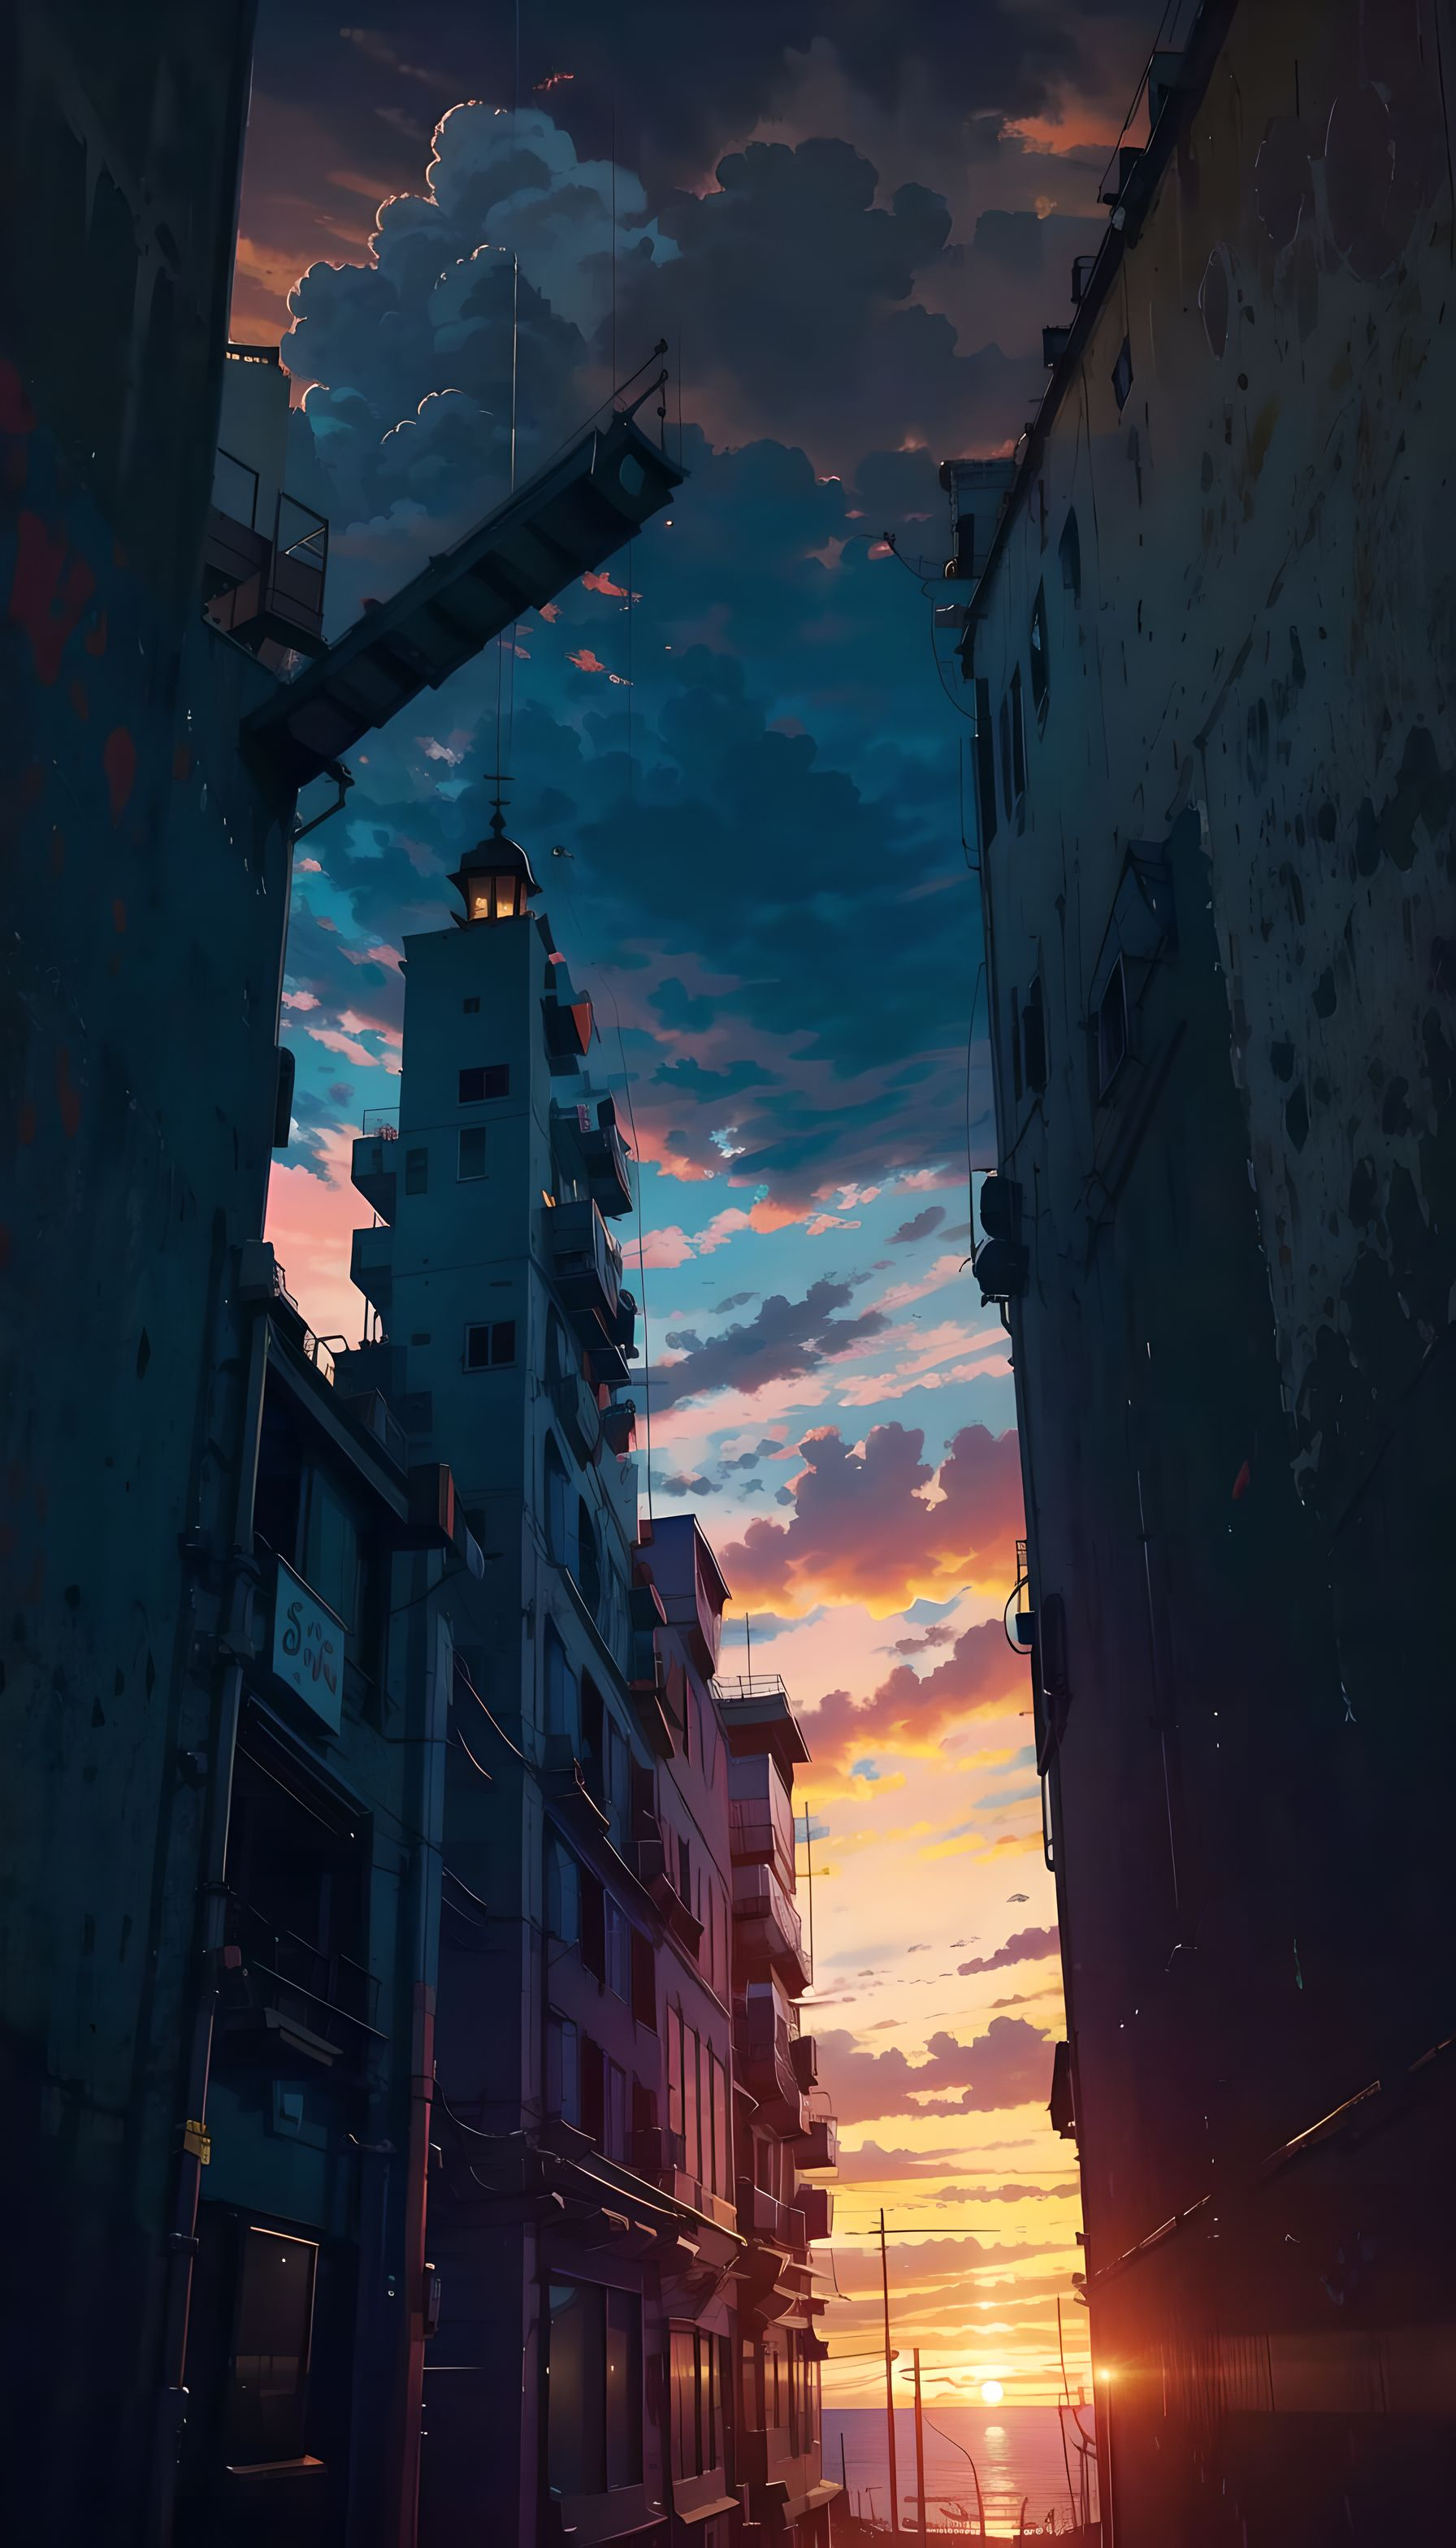
\includegraphics[width=13.5cm]{image/017.jpeg}
\end{center}

\clearpage

\tableofcontents
\listoffigures
\listoftables

\mainmatter
\nocite{*}

\chapter{栅格图像}
通常而言,图像可以分为两类
\begin{itemize}
    \item 栅格图像(Raster Image)是指通过像素阵列描述的图像。
    \item 矢量图像(Vector Image)是指通过几何图元描述的图像。
\end{itemize}

栅格图像的概念非常重要。因为现实中,包括相机、显示屏、打印机等与图像有关的输入输出设备本质上都是栅格设备,它们的“像素”分别是感光元件、发光元件、墨滴。当然,矢量图像也有其自身的优势,由于其本质上存储的是对图形的描述“这里有一个半径多少的圆,那里有一个参数为多少的贝塞尔曲线”,矢量图形是分辨率无关的,在很高分辨率的显示设备上仍然能保持清晰,故很适合用于字体和标志这样的场合。然而,矢量图形在任何显示器上显示前都需要栅格化,介于显示器是栅格设备。除此之外,矢量图形也不可能用于存储相机照片。

\section{栅格设备}

\subsection{输出设备}

图像输出设备可以分为两类:显示(输出到屏幕)和打印(输出到纸张)。

显示主要有两种方式
\begin{itemize}
    \item 透射式(Transmissive):LCD显示(Liquid Crystal Display),基于液晶。
    \item 发射式(Emissive):LED显示(Light Emitting Diode),基于发光二极管。
\end{itemize}
显示屏是由固定的像素阵列组成的,每个像素可以控制其发光强度,对于彩色显示,如\xref{fig:彩色显示的原理}所示,其每个像素将具有三个颜色分别为红、绿、蓝的子像素,当距屏幕一定距离时,我们无法分辨出子像素,而是会看到混合出的颜色。这样控制红、绿、蓝的发光强度就可以控制颜色。

\begin{Figure}[彩色显示的原理]
    \includegraphics[scale=0.8]{build/Chapter03A_01.fig.pdf}
\end{Figure}

在LED显示中,每个像素点就是一个发光二极管,这里展示的共阳极接法,即将所有二极管的正端接在一起并加正电压,此时,阴极接负电压则像素点亮,阴极接正电压则像素熄灭。

\begin{Figure}[LED显示]
    \includegraphics[scale=0.8]{build/Chapter03A_04.fig.pdf}
\end{Figure}

在LCD显示中,每个像素点本身不会发光,而是采用背光显示。在整个屏幕的底部有一块背光(Backlight)作为光源,像素将通过阻挡背光通过实现该像素的熄灭。具体来说,光会首先通过水平偏振镜,从非偏振光变为偏振光。随后,水平偏振光将通过液晶。液晶是一种具有特殊性质的物质,当液晶不加电压时,光将直接通过,当液晶加电压时,光在通过时偏振状态会旋转$\pi/2$,这个例子中,光将会从水平偏振变为垂直偏振。在整个屏幕前部,还有一个垂直偏振镜,它会阻挡水平偏振光的通过但不影响垂直偏振光,故只有液晶通电的像素才会被点亮。
\begin{Figure}[LED显示]
    \includegraphics[scale=0.8]{build/Chapter03A_03.fig.pdf}
\end{Figure}

打印机有很多不同结构的,最常用的是喷墨打印机(Ink Jet Printer),喷墨打印机中有一个载有墨水的墨盒,墨盒的喷嘴可以在电的控制下喷出非常小的墨滴,随着墨盒的移动,最终在纸张上留下图案。彩色打印机需要若干墨水颜色不同的墨盒,墨水在纸张上混合形成各种颜色。

打印机和显示屏的一个区别在于,它没有物理上存在的像素阵列,它的分辨率取决于墨滴可以有多小,因此,和显示屏不同,打印机的分辨率(Resolution)应该使用像素密度而不是像素的总数描述。像素密度(Pixel Denisty)的单位是$\si{dpi}$,即dots per inch。例如称一个打印机的分辨率为$\SI{1200}{dpi}$的意思就是其能在$\SI{1}{inch}\times\SI{1}{inch}$的区域内产生$1200\times 1200$个墨滴。

\subsection{输入设备}
图像输入设备的代表就是相机。相机的核心是图像传感器,类似显示屏,图像传感器也是一个像素阵列,但其每个像素都是一个半导体感光元件。图像传感器主要有两种不同技术
\begin{itemize}
    \item CCD(Charge Coupled Devices)
    \item CMOS(Complimentary Metal Oxide Semiconductor)
\end{itemize}
\begin{Figure}[彩色图像传感器的原理]
    \includegraphics[scale=0.8]{build/Chapter03A_02.fig.pdf}
\end{Figure}
图像传感器实现彩色的方式和显示器类似,在感光元件前加装红、绿、蓝的滤光片,这样一来该感光元件就只能感应该颜色的光了。然而,图像传感器和显示器的一个很大的不同的是,显示器的一个像素包含了三种不同颜色的子像素,图像传感器的一个像素就是一个特定颜色的像素,如\xref{fig:彩色图像传感器的原理}所示。这种滤镜结构称为拜尔滤镜(Bayer Filter),当最终产生图像的时候,由于每个像素只有一个颜色的数据,会参考临近颜色不同的像素的数据补齐颜色信息,该过程称为反马赛克(Demosaicking)。另外,注意到在拜尔滤镜中各颜色像素的数量是不一样的,每个$2\times 2$的像素阵列中,有$1$个红色、$2$个绿色、$1$个蓝色,这是模拟了人眼对绿光最为敏感。

\section{栅格图像}
在了解栅格设备后,本节我们将讨论有关栅格图像的若干问题。

\subsection{栅格图像的数学建模}
首先我们来讨论连续图像,连续图像可以视为这样一个映射
\begin{Equation}
    I(x,y): R\to V
\end{Equation}
\begin{itemize}
    \item $R$是图像存在的一个矩形区域,因此有$R\subset \R^2$。
    \item $V$是图像像素可能的取值范围,对于灰度图像$V\subset\R^{+}$,对于彩色图像$V\subset(\R^{+})^3$。
\end{itemize}

连续图像的实质是光强在矩形域上的连续分布。栅格图像的像素实际上采样的就是像素所在的小区域上光强的平均值,如\xref{fig:栅格图像的建模}所示,这里有必要明确的是像素的排列顺序,使用$(i,j)$表示第$i$列第$j$行的像素,列自左向右,行自下至上。请注意,用$i$表示列用$j$表示行的设定和通常的习惯是相反的!但这样做有一个好处,即$i,j$可以直接与$x,y$对应,转换时不用颠倒。

% 像素坐标$(i,j)$代表了该像素点的中心位置,若总共有$n_x$列$n_y$行像素,则图像的定义域$R=[-0.5,n_x-0.5]\times [-0.5,n_y-0.5]$。

\begin{Figure}[栅格图像的建模]
    \includegraphics[scale=0.8]{build/Chapter03B_05.fig.pdf}
\end{Figure}

设栅格图像共有$n_x$列和$n_y$行像素,则图像中像素$(i,j)$的坐标是
\begin{Gather}
    x=x_l+(x_r-x_l)(i+0.5)/n_x\\
    y=y_b+(y_t-y_b)(j+0.5)/n_y
\end{Gather}
其中$x_l,x_r,y_b,y_t$是图像的左、右、下、上的边界位置。

\subsection{栅格图像的像素值}
我们知道,在计算机中颜色是通过红、绿、蓝即RGB三种颜色以不同比例混合而成的,如果要考虑到颜色的透明度,那还需要添加一个额外的Alpha通道即所谓RGBA。但现在有一个问题,即对于每一种颜色的亮度,我们应当如何量化呢?下面给出两种不同的方法。

高动态范围(HDR, High Dynamic Range),使用浮点数来表示亮度
\begin{Equation}
    I=a\times 2^b
\end{Equation}
低动态范围(LDR, Low Dynamic Range),使用整数来表示亮度
\begin{Equation}
    I=Mc
\end{Equation}
这里$M$表示一个最大亮度(这可能代表显示器能发出或相机能分辨的最亮的光),而$c\in[0,1]$代表一个相对于$M$的亮度,存储时会用以整数表示$c$在$[0,1]$中的分度值,例如假设我们用一个$\SI{8}{bit}$的整数量化,则$0,1,2,\cdots,255$相应表示$c=0,1/255,2/255,\cdots,1$。总结起来说,低动态围就是选定一个亮度范围并用整数表达该范围内一系列均匀间隔的亮度点,高动态范围则是利用浮点数的特性,低亮度下间隔较密,高亮度下间隔较疏但可以动态扩展出很大的亮度范围。实践中,使用整数表示每种颜色的亮度的做法是比较常见的,通常在计算机内部用的就是$\SI{8}{bit}$颜色,故一个RGBA颜色会占用$\SI{32}{bit}$的长度,这刚好是$\SI{32}{bit}$硬件一个字的长度。对于一些专业相机,也会使用$\SI{14}{bit}$或$\SI{16}{bit}$图像以追求照片更为细腻的颜色表现。

容易想象,若设RGB颜色的坐标为$(c_r,c_g,c_b)$,那么所有的颜色都将存在于$V=[0,1]^3$的立方体空间内,在\xref{tab:RGB颜色}中,我们列出了八种最基本的RGB颜色,它们是立方体的八个顶点。

\begin{Tablex}[RGB颜色]{llXrc}
    <颜色中文&颜色英文&备注&坐标&颜色\\>
    黑色&Black&--&$(0,0,0)$&\xcell<c>[1ex][0ex]{\tikz\draw[fill=black] (-0.25,-0.25) rectangle (0.25,0.25);}\\
    红色&Red&--&$(1,0,0)$&\xcell<c>[1ex][0ex]{\tikz\draw[fill=red] (-0.25,-0.25) rectangle (0.25,0.25);}\\
    绿色&Green&--&$(0,1,0)$&\xcell<c>[1ex][0ex]{\tikz\draw[fill=green] (-0.25,-0.25) rectangle (0.25,0.25);}\\
    蓝色&Blue&--&$(0,0,1)$&\xcell<c>[1ex][0ex]{\tikz\draw[fill=blue] (-0.25,-0.25) rectangle (0.25,0.25);}\\
    青色&Cyan&绿和蓝的混合&$(0,1,1)$&\xcell<c>[1ex][0ex]{\tikz\draw[fill=cyan] (-0.25,-0.25) rectangle (0.25,0.25);}\\
    紫色&Magenta&蓝和红的混合~也称为“品红”或“洋红”&$(1,0,1)$&\xcell<c>[1ex][0ex]{\tikz\draw[fill=magenta] (-0.25,-0.25) rectangle (0.25,0.25);}\\
    黄色&Yellow&红和绿的混合&$(1,1,0)$&\xcell<c>[1ex][0ex]{\tikz\draw[fill=yellow] (-0.25,-0.25) rectangle (0.25,0.25);}\\
    白色&White&---&$(1,1,1)$&\xcell<c>[1ex][0ex]{\tikz\draw[fill=white] (-0.25,-0.25) rectangle (0.25,0.25);}\\
\end{Tablex}

当我们讨论透明度的影响时,必须有前景(Foreground)和背景(Background)两张图像。假设前景和后景同一位置的像素的某一颜色分量为$c_f$和$c_b$,且前景该像素透明度为$\alpha$,则
\begin{BoxFormula}[透明度时的叠加公式]
    前后景叠加后的颜色可以表示为
    \begin{Equation}
        c=\alpha c_f+(1-\alpha)c_b
    \end{Equation}
\end{BoxFormula}\goodbreak
我们关注两个边界情况
\begin{itemize}
    \item 当前景$\alpha=0$,有$\alpha=c_b$成立,即意味着前景“完全透明”。
    \item 当前景$\alpha=1$,有$\alpha=c_f$成立,即意味着前景“完全不透明”。
\end{itemize}
这意味着,如果我们希望在RGBA下表示不透明的颜色,我们应当令$\alpha=1$(而不是反之)。

\subsection{显示与伽马校正}
若一个像素的值为$a\in[0,1]$,显示屏最大亮度为$M$,显示屏该像素处的亮度应当为
\begin{Equation}
    I=Ma
\end{Equation}

但实际上,并不是如此,因为显示屏的输入和输出之间存在非线性的关系!这种非线性关系可以近似为幂函数,幂函数的指数用$\gamma$表示,这是一个与显示屏特性有关的量
\begin{Equation}
    I=Ma^{\gamma}
\end{Equation}

\xref{fig:伽马值对显示的影响}展示了$\gamma$的影响,对于当下典型的显示屏,有$\gamma=2.2$。
\begin{Figure}[伽马值对显示的影响]
    \includegraphics[scale=0.8]{build/Chapter03B_07a.fig.pdf}
\end{Figure}

现在的问题是,我们如何测定一个显示屏的$\gamma$值?如\xref{fig:伽马值的测定方法}所示,我们令显示屏显示左侧这样的黑白相间的棋盘图案,假如这种图案足够密集,那从远处看就是灰色的,而且由于这种灰色是通过一半白一半黑直接在空间上混合出来的,我们可以确定其$I/M=0.5$。同时,我们在右侧显示一个值为$a$的纯色,调节$a$的值使左右看起来一致,此时有下式成立
\begin{Equation}
    a^{\gamma}=0.5
\end{Equation}

这样一来
\begin{Equation}
    \gamma=\frac{\ln 0.5}{\ln a}
\end{Equation}

\begin{Figure}[伽马值的测定方法]
    \includegraphics[scale=0.8]{build/Chapter03B_03.fig.pdf}
\end{Figure}

假如我们已知知道$\gamma$,为了消除其影响,可以在输出之前通过$a'=a^{1/\gamma}$进行矫正。

\begin{Figure}[灰度色阶的对比]
    \begin{FigureSub}[校正前]
        \includegraphics[scale=0.8]{build/Chapter03B_01.fig.pdf}
    \end{FigureSub}\\ \vspace{0.25cm}
    \begin{FigureSub}[校正后]
        \includegraphics[scale=0.8]{build/Chapter03B_02.fig.pdf}
    \end{FigureSub}
\end{Figure}

这里有一个问题,为什么显示屏不能设法令$\gamma=1$?在早期CRT显示器的年代,输出和输入确实是存在物理上的非线性关系,而现代的显示器其实是完全线性的,前面提到的$\gamma=2.2$其实是人为引入的!这样做的目的可以通过\xref{fig:灰度色阶的对比}所示的一个小实验理解,\xref{fig:校正前}是未校正的色阶,\xref{fig:校正后}是依照$\gamma=2.2$下$a'=a^{1/\gamma}$校正后的色阶,我们会注意到,校正后的灰度色阶人眼看起来反而没有那么均匀了,但如果我们用仪器测量光强,校正后的光强其实是线性分布的,这是怎么回事?实际上,人眼对于光强的感知是非线性的,简单来说,我们感知的其实是光强的数量级而不是绝对值。而显示屏$\gamma=2.2$恰恰就是为了补偿人眼的非线性,这个数值是通过大量试验得出的。所以如果目标是追求视觉上的适当,无需进行$a'=a^{1/\gamma}$的修正。
\chapter{光线追踪}

计算机图形学的一个基本任务就是三维场景的渲染(Redering)。渲染是指,对于一系列排列在三维空间中的物体,产生一张从三维空间特定视角观察这些物体的二维图像。本质上说,渲染是一系列物体为输入以一个像素阵列为输出的过程,无论具体如何实现,渲染总会涉及这样一个问题:每个物体是如何影响每个像素的?渲染有以下两种的主流实现方式
\begin{enumerate}
    \item 物体顺序渲染(Object Order Redering),遍历每个物体,考虑它们会影响哪些像素。
    \item 图像顺序渲染(Image Order Redering),遍历每个像素,考虑它们将如何被物体确定。
\end{enumerate}
若借用计算机语言,渲染即是一个包含遍历物体和遍历像素的双重循环,物体顺序渲染和图像顺序渲染的差别就是哪一循环在外面。两种渲染方式都可以产生相同的图像,但是效率和复杂性是不同的。通常而言,图像顺序渲染更简单也更灵活,不过相较物体顺序渲染需要更长的时间来产生一张图像。本章将研究的光线追踪(Ray Tracking)是一种图像顺序渲染算法。

\section{光线追踪的基本概念}

光线追踪的基本概念可以用\xref{fig:光线追踪的基本概念}来说明,对于每个像素,我们将会产生一条光线,光线的原点和方向与选取的投影方式有关。光线会在三维空间中穿行,光线第一个遇到的物体就代表该像素“看到”的是这个物体,像素就会被渲染为这个物体的颜色。例如在\xref{fig:光线追踪的基本概念}中光线追踪到的是三角面$T_1$。三角面$T_2$未被光线经过,三角面$T_3$在光线上但$T_1$在其前面先遇到光线了。
\begin{Figure}[光线追踪的基本概念]
    \includegraphics[scale=0.8]{build/Chapter04B_03.fig.pdf}
\end{Figure}

因此,简单来说,光线追踪可以分为两个步骤
\begin{enumerate}
    \item 光线产生(Ray Generation),确定每个像素对应的光线的原点和方向。
    \item 光线相交(Ray Intersection),找到最近的与光线相交的物体。
\end{enumerate}
\section{光线产生}
光线产生和投影方式有关,主要有以下两种投影
\begin{itemize}
    \item 平行投影(Parallel Projection),如\cref{fig:平行投影}所示,是指光线从每个像素的中心处发出且所有光线是平行的。平行投影可以分为两种情况,取决于光线方向是否与像平面垂直,分别称为正交投影(Orthographic)和斜交投影(Oblique),其中正交投影比较常见,我们在\cref{fig:平行投影}展示的也是正交投影的情况。平行投影常用于工程图(例如机械和建筑)的绘制,它的最大特征是,三维空间中的平行线经过投影后在二维图像中仍然是平行的。
    \item 透视投影(Perspective Projection),如\cref{fig:透视投影}所示,是指光线从一个特定的观察点处向各个像素的方向发出,观察点位于像平面中心后方处。透视投影符合人眼或相机的成像模式,它的特点是具有透视效应,近大远小,平行线不一定再平行。试想,站在一条笔直的公路中央望向远方,会发现公路两侧边沿会逐渐靠拢,但它们实际是平行的。
\end{itemize}

\begin{Figure}[两种投影方式]
    \figuresub[平行投影]{\includegraphics[scale=0.8]{Chapter04B_01.fig.pdf}}    
    \figuresub[透视投影]{\includegraphics[scale=0.8]{Chapter04B_02.fig.pdf}}    
\end{Figure}

有趣的是,平行投影在一定意义上可以认为是观察点位于无穷远处的透视投影。这一理解最直观的感受是,长焦镜头具有压缩空间的效果,即透视带来的近大远小在长焦下不太明显了。

在\cref{fig:两种投影方式}中,有一些标注需要说明。首先,无论是平行投影还是透视投影,我们都会确定一个原点$\vb{e}$,对于平行投影是像平面中心,对于透视投影是观察点。其次,在$\vb{e}$上标注了三个重要的单位矢量$\vb{u},\vb{v},\vb{w}$,三者呈右手螺旋关系。其中,$\vb{w}$是视野方向的反方向,$\vb{v},\vb{u}$均位于像平面,它们会定义画面的“上”和“右”在空间中的对应方向。最后,$u_l,u_r,v_b,v_t$分别确定了画面在左、右、下、上的边界。特别的,在透视投影中,$d$还用于表示观察点和像平面间的距离。

假设二维图像的像素总数是$n_x\times n_y$,对于$(i,j)$处的像素,其水平位置$u$和垂直位置$v$为
\begin{Gather}
    u=x_l+(x_r-x_l)(i+0.5)/n_x\\
    v=y_b+(y_t-y_b)(j+0.5)/n_y
\end{Gather}

我们可以用一个参数方程表达三维空间的直线(即这里的光线)
\begin{BoxDefinition}[三维直线的参数方程]
    三维空间中的直线遵循以下参数方程
    \begin{Equation}
        \vb{p}(t)=\vb{e}+\vb{d}t
    \end{Equation}
\end{BoxDefinition}

其中,$\vb{e}$代表光线的原点,$\vb{d}$代表光线的方向。应指出的是光线的原点$\vb{e}$未必是\cref{fig:两种投影方式}中投影的原点$\vb{e}$,为强调这一区别,在本小节将光线方程$\vb{p}(t)=\vb{e}+\vb{d}t$中的$\vb{e},\vb{d}$记为$\vb{e}_{ray},\vb{d}_{ray}$。

对于平行投影,光线的原点在变化,但方向不变
\begin{BoxFormula}[平行投影的光线方程]
    平行投影的光线方程,原点$\vb{e}_{ray}$和方向$\vb{d}_{ray}$分别为
    \begin{Gather}
        \vb{e}_{ray}=\vb{e}+u\vb{u}+v\vb{v}\\
        \vb{d}_{ray}=-\vb{w}
    \end{Gather}
\end{BoxFormula}

对于透视投影,光线的方向在变化,但原点不变
\begin{BoxFormula}[透视投影的光线方程]
    透视投影的光线方程,原点$\vb{e}_{ray}$和方向$\vb{d}_{ray}$分别为
    \begin{Gather}
        \vb{e}_{ray}=\vb{e}\\
        \vb{d}_{ray}=-\vb{d}\vb{w}+u\vb{u}+v\vb{v}
    \end{Gather}
\end{BoxFormula}
\section{光线相交}
由于实际的三维模型都是由其表面一系列的三角面组成的,因此,我们唯一要处理的和光线相交的物体就是三角面。和光线的表示类似,三角面也可以用参数方程的方式表达
\begin{BoxDefinition}[三角面的参数方程]
    三角面遵循以下参数方程
    \begin{Equation}
        \vb{f}(\beta,\gamma)=\vb{a}+\beta(\vb{b}-\vb{a})+\gamma(\vb{c}-\vb{a})
    \end{Equation}
\end{BoxDefinition}

其中,$\vb{a},\vb{b},\vb{c}$为三角面的三个顶点,$\beta,\gamma$是参数满足$\beta>0,\gamma>0$以及$\beta+\gamma<1$,这个范围是为了保证点位于三角面内部,因为$\vb{a}+\beta(\vb{b}-\vb{a})+\gamma(\vb{c}-\vb{a})$本身表示的是一整个平面。

现在联立$\vb{p}(t)=\vb{f}(\beta,\gamma)$,代入\xref{def:三维直线的参数方程}和\xref{def:三角面的参数方程},

\begin{Equation}&[1]
    \vb{e}+\vb{d}t=\vb{a}+\beta(\vb{b}-\vb{a})+\gamma(\vb{c}-\vb{a})
\end{Equation}
将$\vb{e},\vb{d}$和$\vb{a},\vb{b},\vb{c}$展开
\begin{Align}
    x_e+tx_d&=x_a+\beta(x_b-x_a)+\gamma(x_c-x_a)\\
    y_e+ty_d&=y_a+\beta(y_b-y_a)+\gamma(y_c-y_a)\\
    z_e+tz_d&=z_a+\beta(z_b-z_a)+\gamma(z_c-z_a)
\end{Align}
我们可以写成标准的矩阵形式
\begin{Equation}
    \begin{pmatrix}
        x_a-x_b&x_a-x_c&x_d\\
        y_a-y_b&y_a-y_c&y_d\\
        z_a-z_b&z_a-z_c&z_d\\
    \end{pmatrix}
    \begin{pmatrix}
        \beta\\
        \gamma\\
        t\\
    \end{pmatrix}=
    \begin{pmatrix}
        x_a-x_e\\
        y_a-y_e\\
        z_a-z_e\\
    \end{pmatrix}
\end{Equation}
这等价于
\begin{Equation}
    \begin{pmatrix}
        \vb{a}-\vb{b}&\vb{a}-\vb{c}&\vb{d}
    \end{pmatrix}
    \begin{pmatrix}
        \beta\\
        \gamma\\
        t
    \end{pmatrix}=
    \begin{pmatrix}
        \vb{a}-\vb{e}
    \end{pmatrix}
\end{Equation}
这个方程可以很容易的通过行列式的相关知识求出结果,至此求交点的问题已经被解决。
% \begin{BoxFormula}[光线和三角面的相交]
%     光线和三角面相交,联立方程为
%     \begin{Equation}
%         \begin{pmatrix}
%             \vb{a}-\vb{b}&\vb{a}-\vb{c}&\vb{d}
%         \end{pmatrix}
%         \begin{pmatrix}
%             \beta\\
%             \gamma\\
%             t
%         \end{pmatrix}=
%         \begin{pmatrix}
%             \vb{a}-\vb{e}
%         \end{pmatrix}
%     \end{Equation}
% \end{BoxFormula}
解出方程后,我们将得到一组$t,\beta,\gamma$,如何判读这个结果?首先,若$\beta,\gamma>0$和$\beta+\gamma<1$不成立,则说明该光线与三角面所在平面的交点并不在三角面内部。其次,应验证$t\in[t_0,t_1]$是否成立,通常而言$t_0=0$而$t_1=+\infty$,我们不希望在视野背后的三角面也被渲染。最后,如果光线与多个三角面存在交点,我们应当渲染的是$t$最小的三角面,因为它在视野中最靠前。

% 这里有一个问题,透视投影中$0\leq t\leq 1$是观察点和像平面间的区域,该区域是否要渲染?
% \section{表面着色}
% 着色(Shading)是指这样一件事,若某条光线追踪到某个物体,那么这条光线对应的像素应该渲染为什么颜色?最朴素的思路是,物体是什么颜色就将像素渲染为什么颜色,这可行但效果肯定不好,试想,这样渲染一个蓝色的球体将得到一个完全是蓝色的圆,毫无立体感。我们知道,物体的立体感来自光源照射下的明暗层次。因此,如果希望渲染结果比较有立体感,我们必须考虑光源的影响!最简单的想法是,正对光的面会比较亮,侧对光的面会比较暗。除此之外,材料还有高光和哑光之分。总而言之,着色研究的就是光源对于物体自身颜色的影响。

% \subsection{着色方程的建立}
% 我们考虑\cref{fig:着色原理}所示的着色过程示意图,先将所有符号说明如下
% \begin{itemize}
%     \item Light表示点光源的位置,在本节考虑的光源暂且都是点状的。
%     \item View表示视线原点的位置,这里的视线就是光线追踪中的光线,只不过由于这里在讨论光源的影响,将由观察点发出的射线再称为“光线”会有歧义,故用“视线”一词。
%     \item 向量$\vb{n}$代表三角面朝外的的单位法向量。
%     \item 向量\hspace{0.47em}$\vb{l}$\hspace{0.47em}代表三角面(与视线交点处)指向光源点的单位向量。
%     \item 向量$\vb{v}$代表三角面(与视线交点处)指向视线原点的单位向量。
%     \item 向量$\vb{h}$代表指向$\vb{v},\vb{l}$角平分线的单位向量,可由$\vb{h}=(\vb{v}+\vb{l})/\norm{\vb{v}+\vb{l}}$得到。
% \end{itemize}
% \begin{Figure}[着色原理]
%     \includegraphics[scale=0.8]{Chapter05C_01.fig.pdf}
% \end{Figure}

% 着色过程可以分成以下三种机制:Lambertian着色、Blinn-Phong着色、Ambient着色。
% \begin{BoxFormula}[Lambertian着色]
%     Lambertian着色表征了点光源的漫反射
%     \begin{Equation}
%         c=c_lc_d\max(0,\vb{n}\cdot\vb{l})
%     \end{Equation}
% \end{BoxFormula}
% \begin{BoxFormula}[Blinn-Phong着色]
%     Blinn-Phong着色表征了点光源的镜面反射
%     \begin{Equation}
%         c=c_lc_s\max(0,\vb{n}\cdot\vb{h})^p
%     \end{Equation}
% \end{BoxFormula}
% \begin{BoxFormula}[Ambient着色]
%     Ambient着色表征了环境光源的漫反射
%     \begin{Equation}
%         c=c_ac_d
%     \end{Equation}
% \end{BoxFormula}

% 这三种着色机制是共同作用的,最终的着色结果是三者之和
% \begin{Equation}
%     c=c_ac_d+c_lc_d\max(0,\vb{n}\cdot\vb{l})+c_lc_s\max(0,\vb{n}\cdot\vb{h})^p
% \end{Equation}

% 接下来,我们将逐步解读这三种着色机制对应的着色方程的物理意义及相关符号的含义。

% \subsection{着色方程的意义}

% 第一步,我们要理解光源照射至物体表面时,存在两种光学过程
% \begin{itemize}
%     \item 漫反射(Diffuse Reflection):光线照射至粗糙表面时会由于表面的不平整而向各个方向反射。这就是说,漫反射向各个方向均匀反射了从光源吸收的能量,因而从任意角度看表面都是完全相同的亮度,换言之,漫反射是视角无关的!那么,漫反射下表面的亮度与什么有关?朴素的观察指出,光垂直照射表面是最亮的,光平行照射表面是最暗的,在数学上,这可以用表面法向量$\vb{n}$与光线向量$\vb{l}$的夹角余弦$\cos\theta$表示,我们可以简单验证这一点:垂直照射$\theta=0$时有$\cos\theta=1$,平行照射$\theta=\pm\pi/2$时有$\cos\theta=0$。当然必须要考虑到的是,亮度不可能小于零,当光线照向了表面的背面时不可能“比黑更黑”,故修改为$\max(0,\cos\theta)$。最后,由于$\vb{n},\vb{l}$均为单位向量,因此可以改写为$\max(0,\vb{n}\cdot\vb{l})$。
%     \item 镜面反射(Specular Reflection):光线照射至较光滑的表面时反射光线会相对集中在镜面反射方向上。换言之,如果视线恰好在反射方向附近,我们将看到更亮的光。而考察视线和反射方向是否重合,其实等价于考察视线和光线的角平分线方向$\vb{h}$是否位于表面法向$\vb{n}$上,因而有了$\max(0,\vb{n}\cdot\vb{h})$,添加一个系数$p>1$即$\max(0,\vb{n}\cdot\vb{h})^p$可以使视线偏离反射方向后亮度以更快的速度衰减至零。系数$p$反映了表面的光滑程度,系数$p$较大则意味着表面较光滑,使反射光线只集中在镜面反射方向附近的一个很小的角度范围内。
% \end{itemize}

% 其中,Lambertian着色和Blinn-Phong着色分别代表了点光源的漫反射和镜面反射。然而若仅考虑这两者会导致一个问题,即背朝光源的表面将是完全黑暗的,这不美观也不符合我们的实际感受。Ambient着色引入了环境光源,环境光源可以认为是弥散在整个环境中各向同性的光源,换言之,环境光源对于每一个表面都是垂直照射的,保障一个最低程度的照明。

% 第二步,我们要理解方程中各颜色$c_l,c_a,c_d,c_s$的含义,所有颜色可以分为两组
% \begin{itemize}
%     \item 光源颜色$c_l,c_a$\hspace{0.15em}:分别代表“点光源颜色”和“环境光源颜色”。
%     \item 物体颜色$c_d,c_s$:分别代表“漫反射颜色”和“镜面反射颜色”。
%     \item 有关符号下标,$c_l,c_a$代表Light和Ambient,$c_d,c_s$代表Diffuse和Specular。
% \end{itemize}
% 而对于一种着色机制,取决于光源类型和反射机制,会带有两项颜色系数
% \begin{itemize}
%     \item Lambertian着色是点光源的漫反射,故有$c=c_lc_d\max(0,\vb{n}\cdot\vb{l})成立$。
%     \item Blinn-Phong着色是点光源的镜面反射,故有$c=c_lc_s\max(0,\vb{n}\cdot\vb{h})^p$成立。
%     \item Ambient着色是环境光源的漫反射(环境光总垂直表面),故有$c=c_ac_d$成立。
% \end{itemize}

% 应当指出,这里$c_l,c_a,c_d,c_s$都应该解读为颜色的某一分量,完整的结果需对于RGB的每一颜色分量重复一遍。这是符合直觉的,白色的光照射在红色物体上我们将只会看到红色。


% 还要注意的是,由于$c\in[0,1]$,为了保证$c$的结果不溢出该范围,需要加一些限制。

% 光源颜色的总和不能超过$1$
% \begin{Equation}
%     c_l+c_a\leq 1
% \end{Equation}
% 物体颜色的总和不能超过$1$
% \begin{Equation}
%     c_d+c_s\leq 1
% \end{Equation}
% 这里我们可能对$c_d+c_s\leq 1$带来的物体颜色无法自由指定感到困惑。但可以这么想,若一个物体需要表现出高光,那它本身的颜色就不可能太亮,否则高光部分又怎么显示出“高光”呢?


% 注意,Lambertian和Blinn-Phong均为人名,但Ambient不是,它的意思就是环境!

% \subsection{着色方程的效果}
% 在本小节,我们将考察一个正交投影下的立方体(12个三角面)在不同着色下的渲染效果。
% \begin{Figure}[Lambertian着色和Ambient着色]
%     \begin{FigureSub}[Lambertian着色]
%         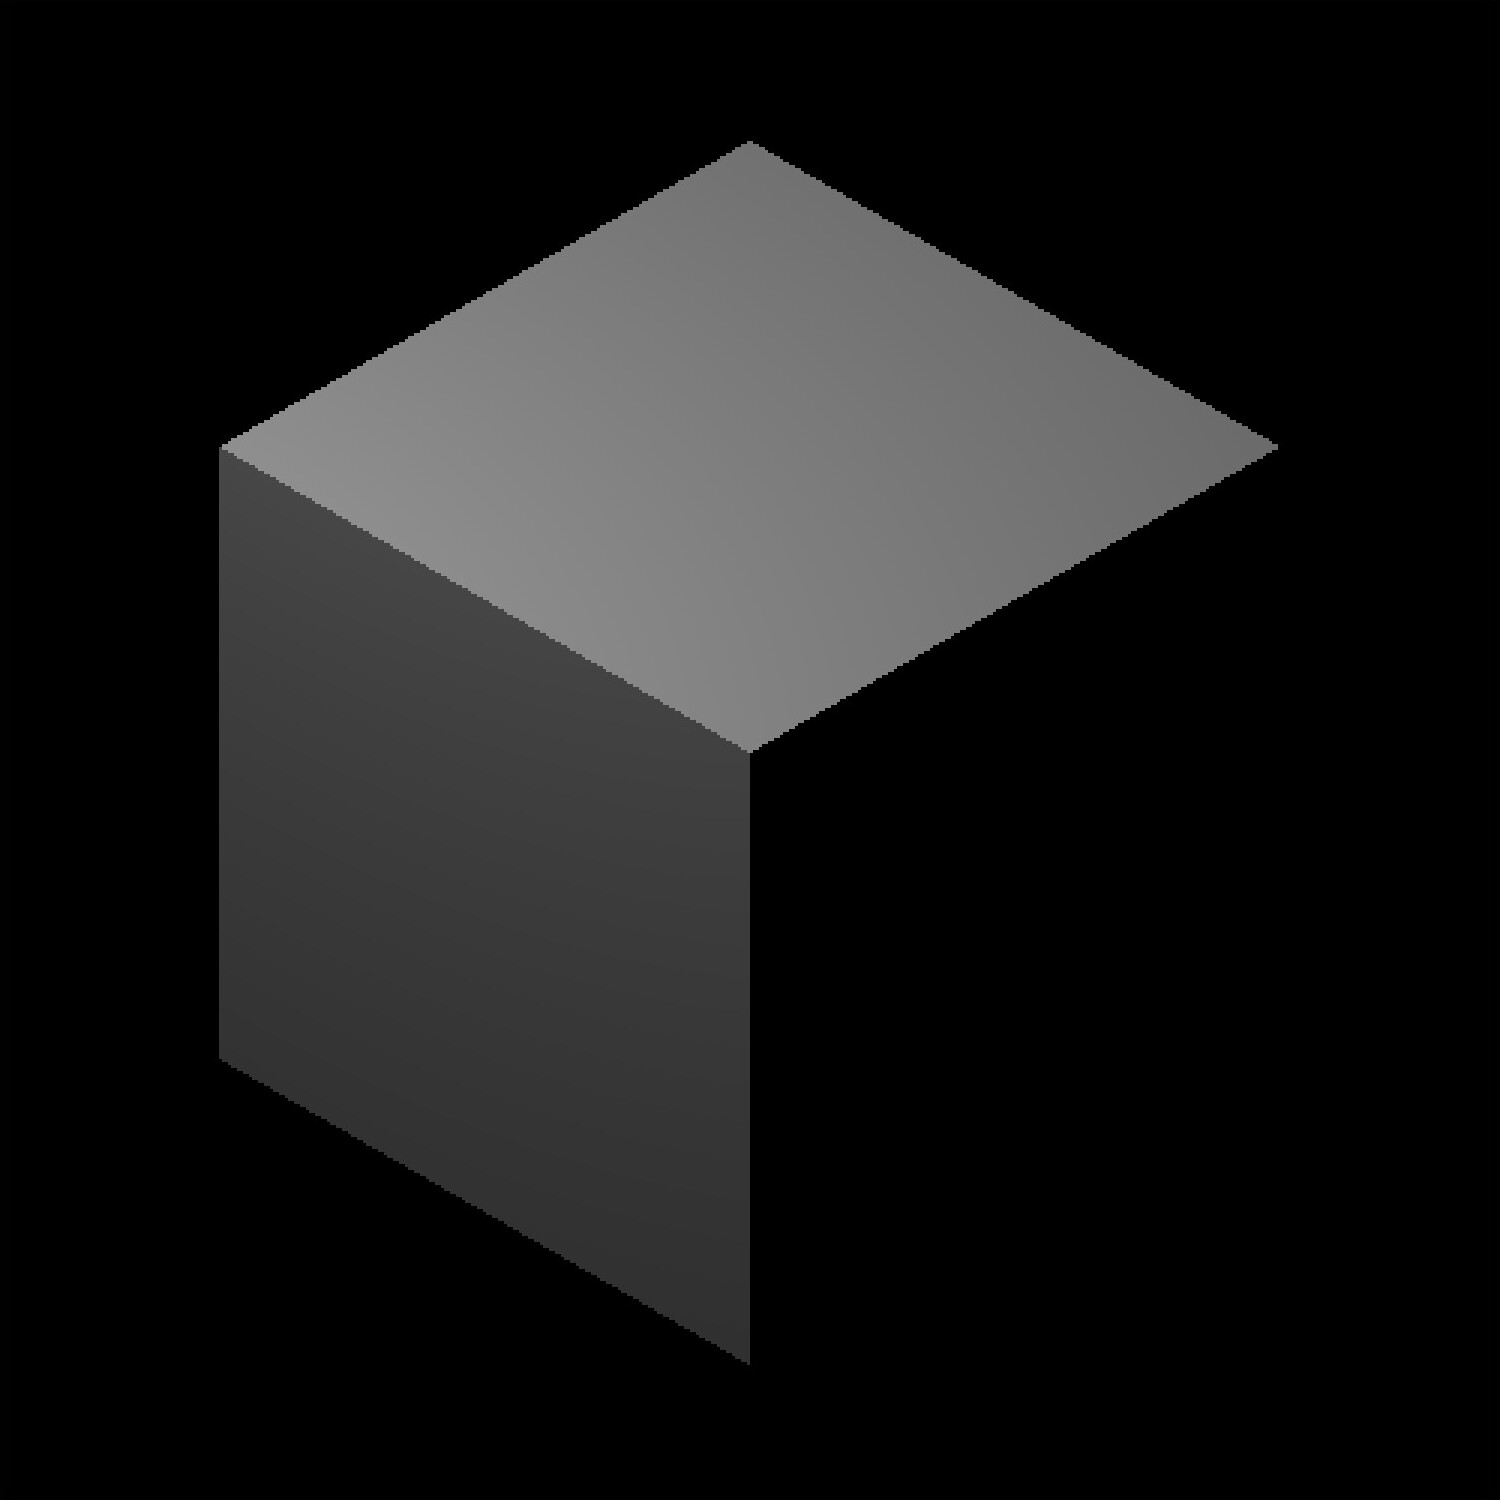
\includegraphics[width=3.8cm]{Cube1.jpg}
%     \end{FigureSub}
%     \hspace{0.5cm}
%     \begin{FigureSub}[Ambient着色]
%         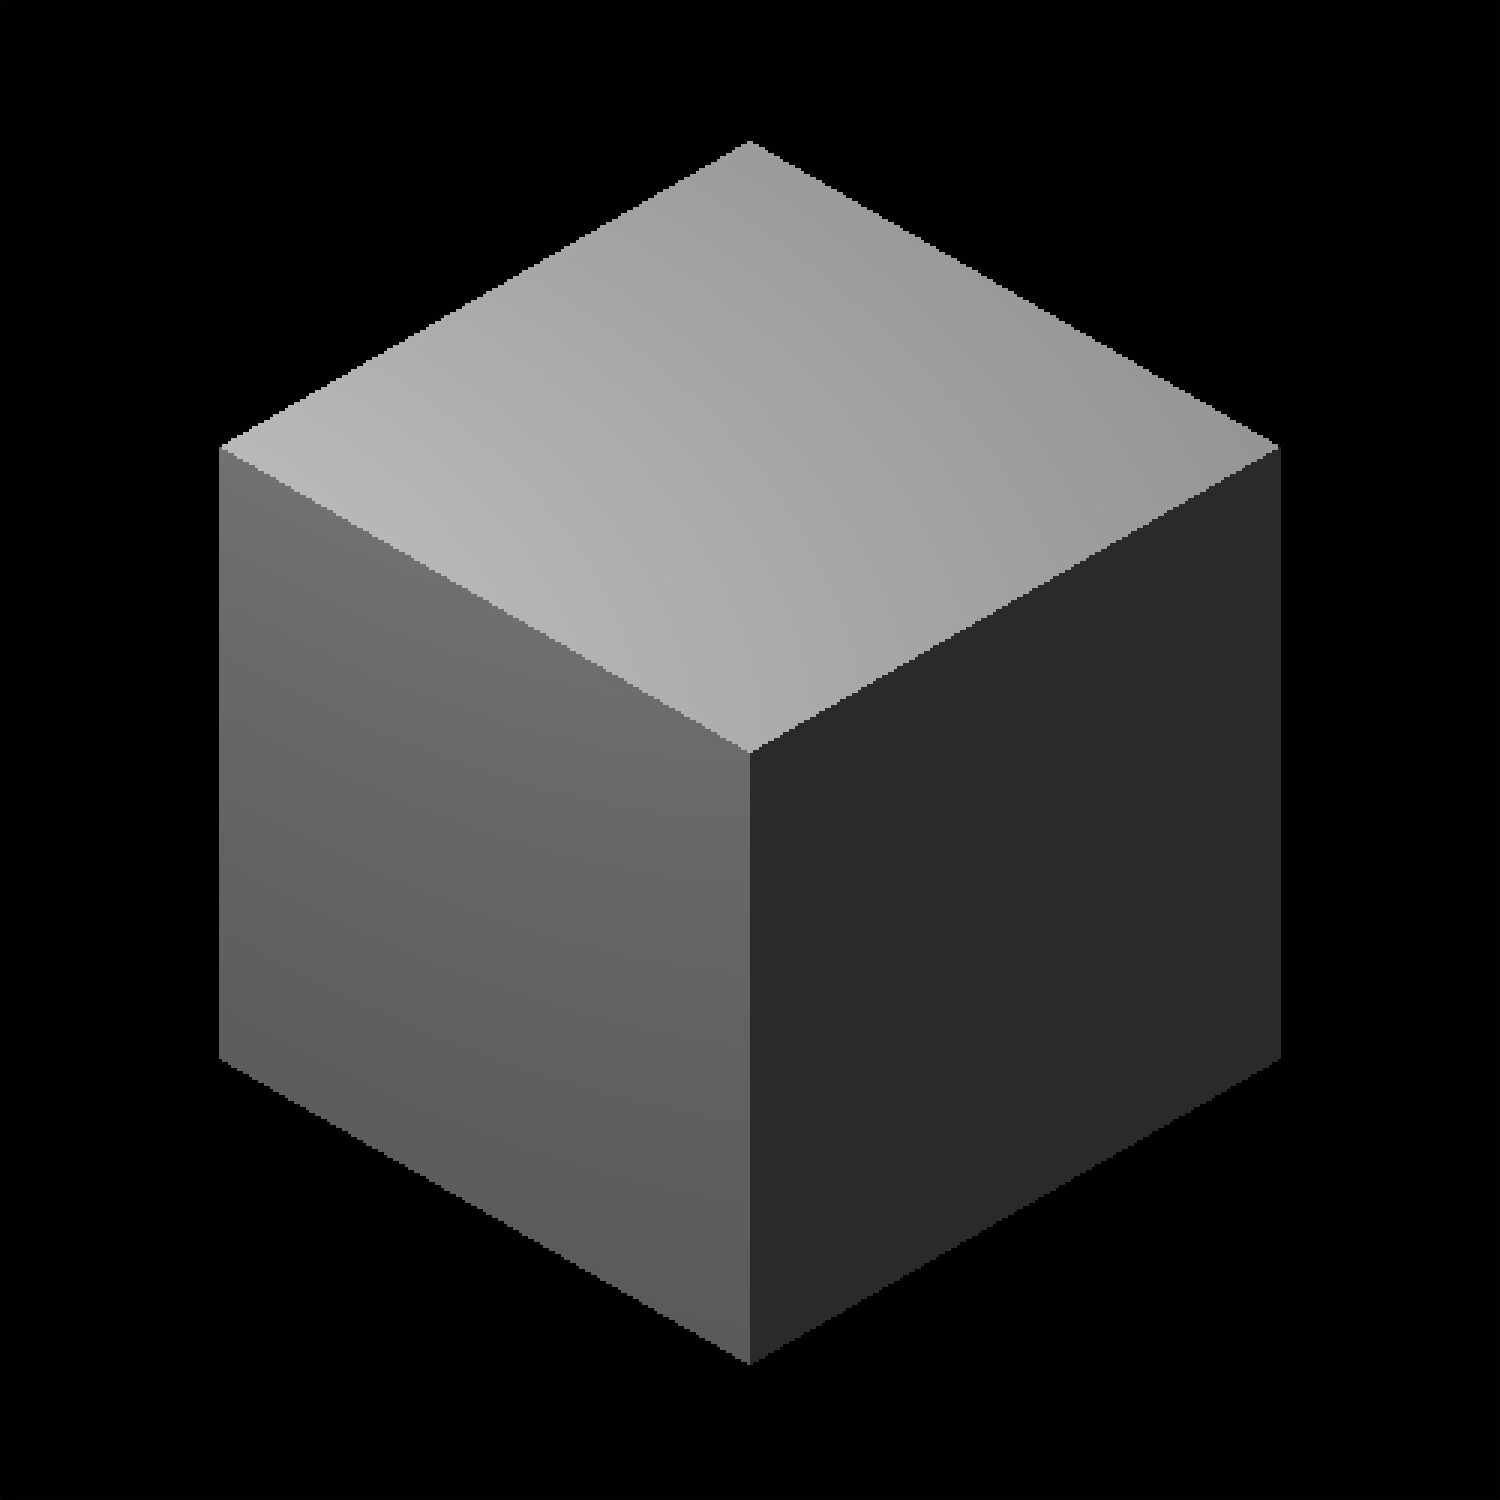
\includegraphics[width=3.8cm]{Cube2.jpg}
%     \end{FigureSub}
% \end{Figure}
% \cref{fig:Lambertian着色}中仅考虑了Lambertian着色,光源从左侧照向立方体。注意到,左侧面和上侧面被不同程度照亮,这是因为光线和左侧面与上侧面的法向量具有不同的夹角,同时,右侧面未被照亮,是全黑的。\cref{fig:Ambient着色}在此基础上添加了Ambient着色,得益于环境光照的引入,右侧面现在不再是完全黑暗的,同时,叠加环境光照后,左侧面和上侧面也比原来更亮了一些。

% \begin{Figure}[Blinn-Phong着色]
%     \begin{FigureSub}[$p=10$;p10]
%         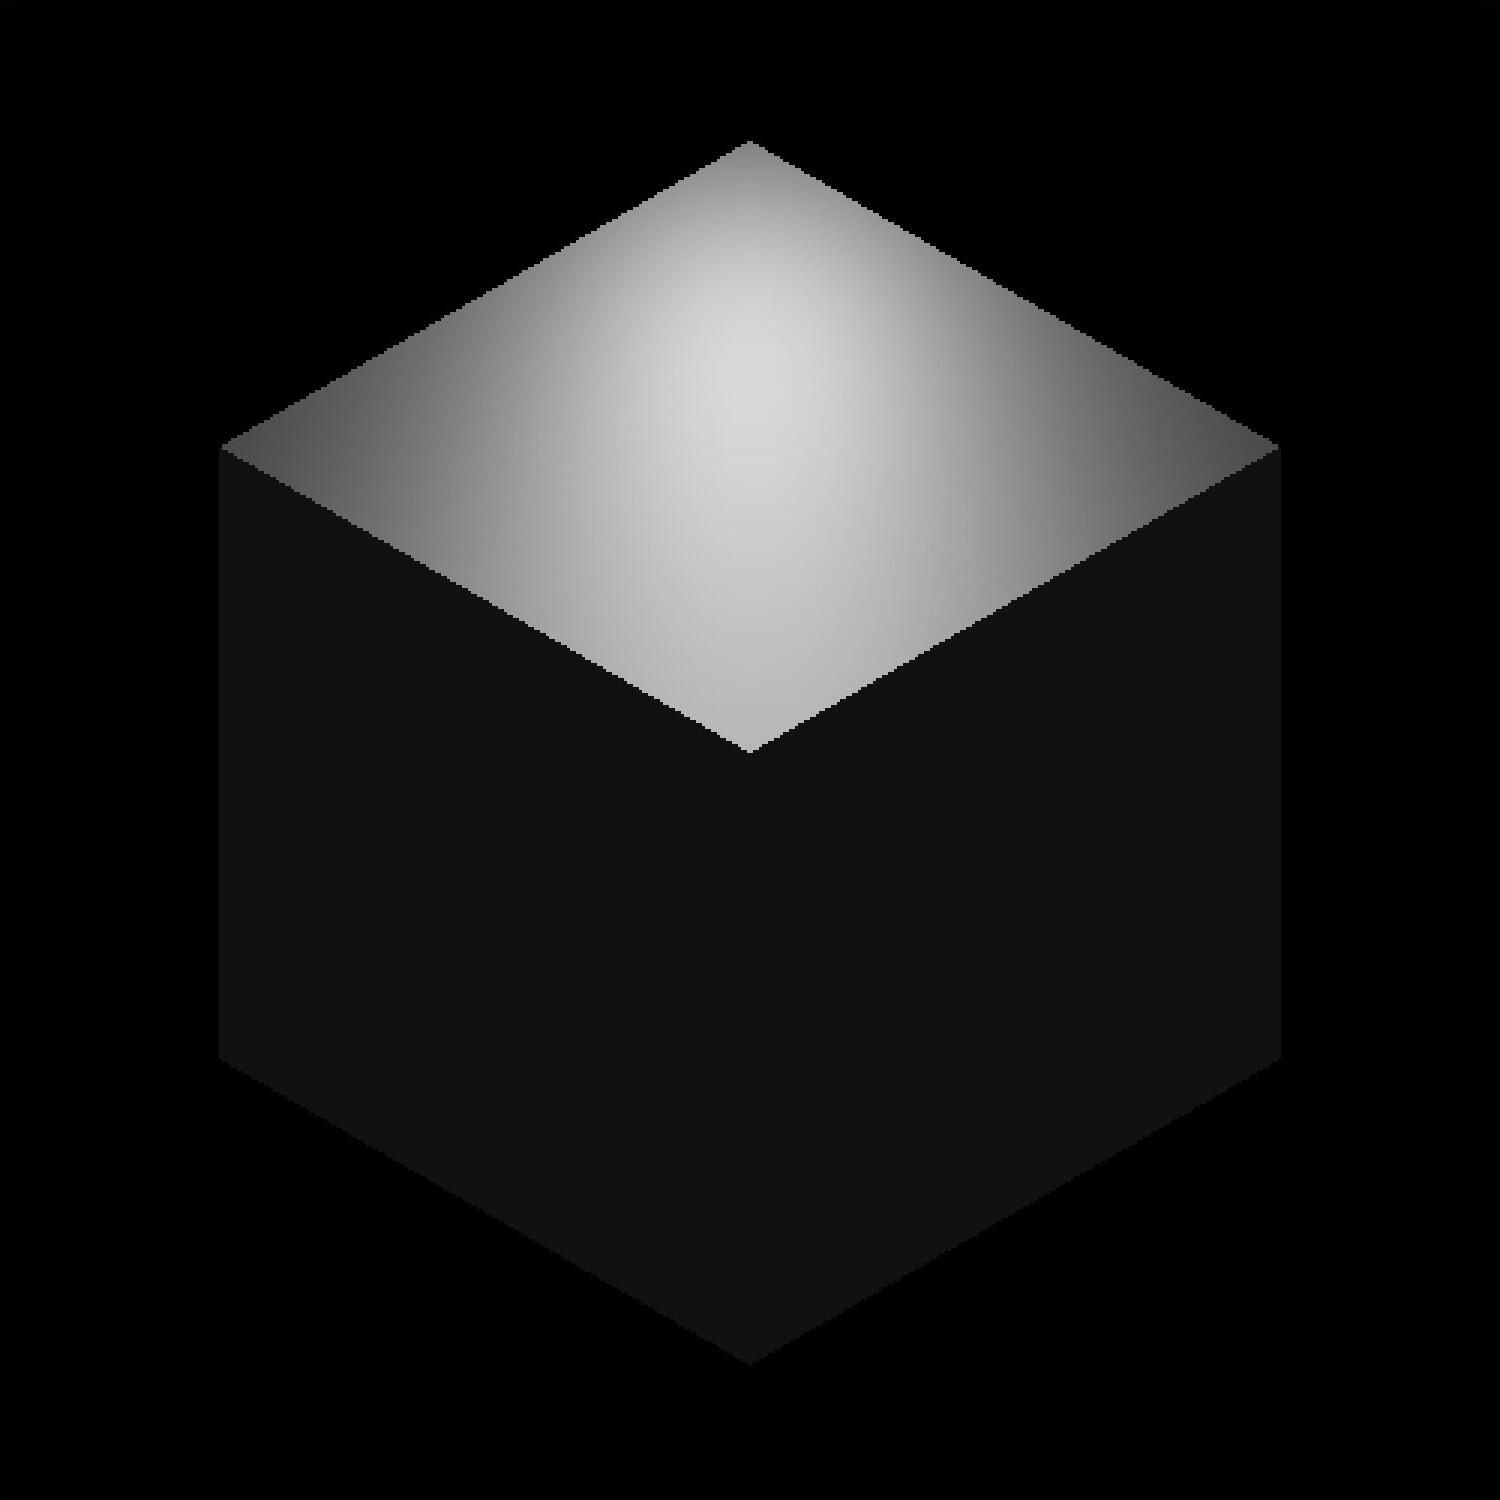
\includegraphics[width=3.8cm]{Cube3.jpg}
%     \end{FigureSub}
%     \hspace{0.5cm}
%     \begin{FigureSub}[$p=100$;p100]
%         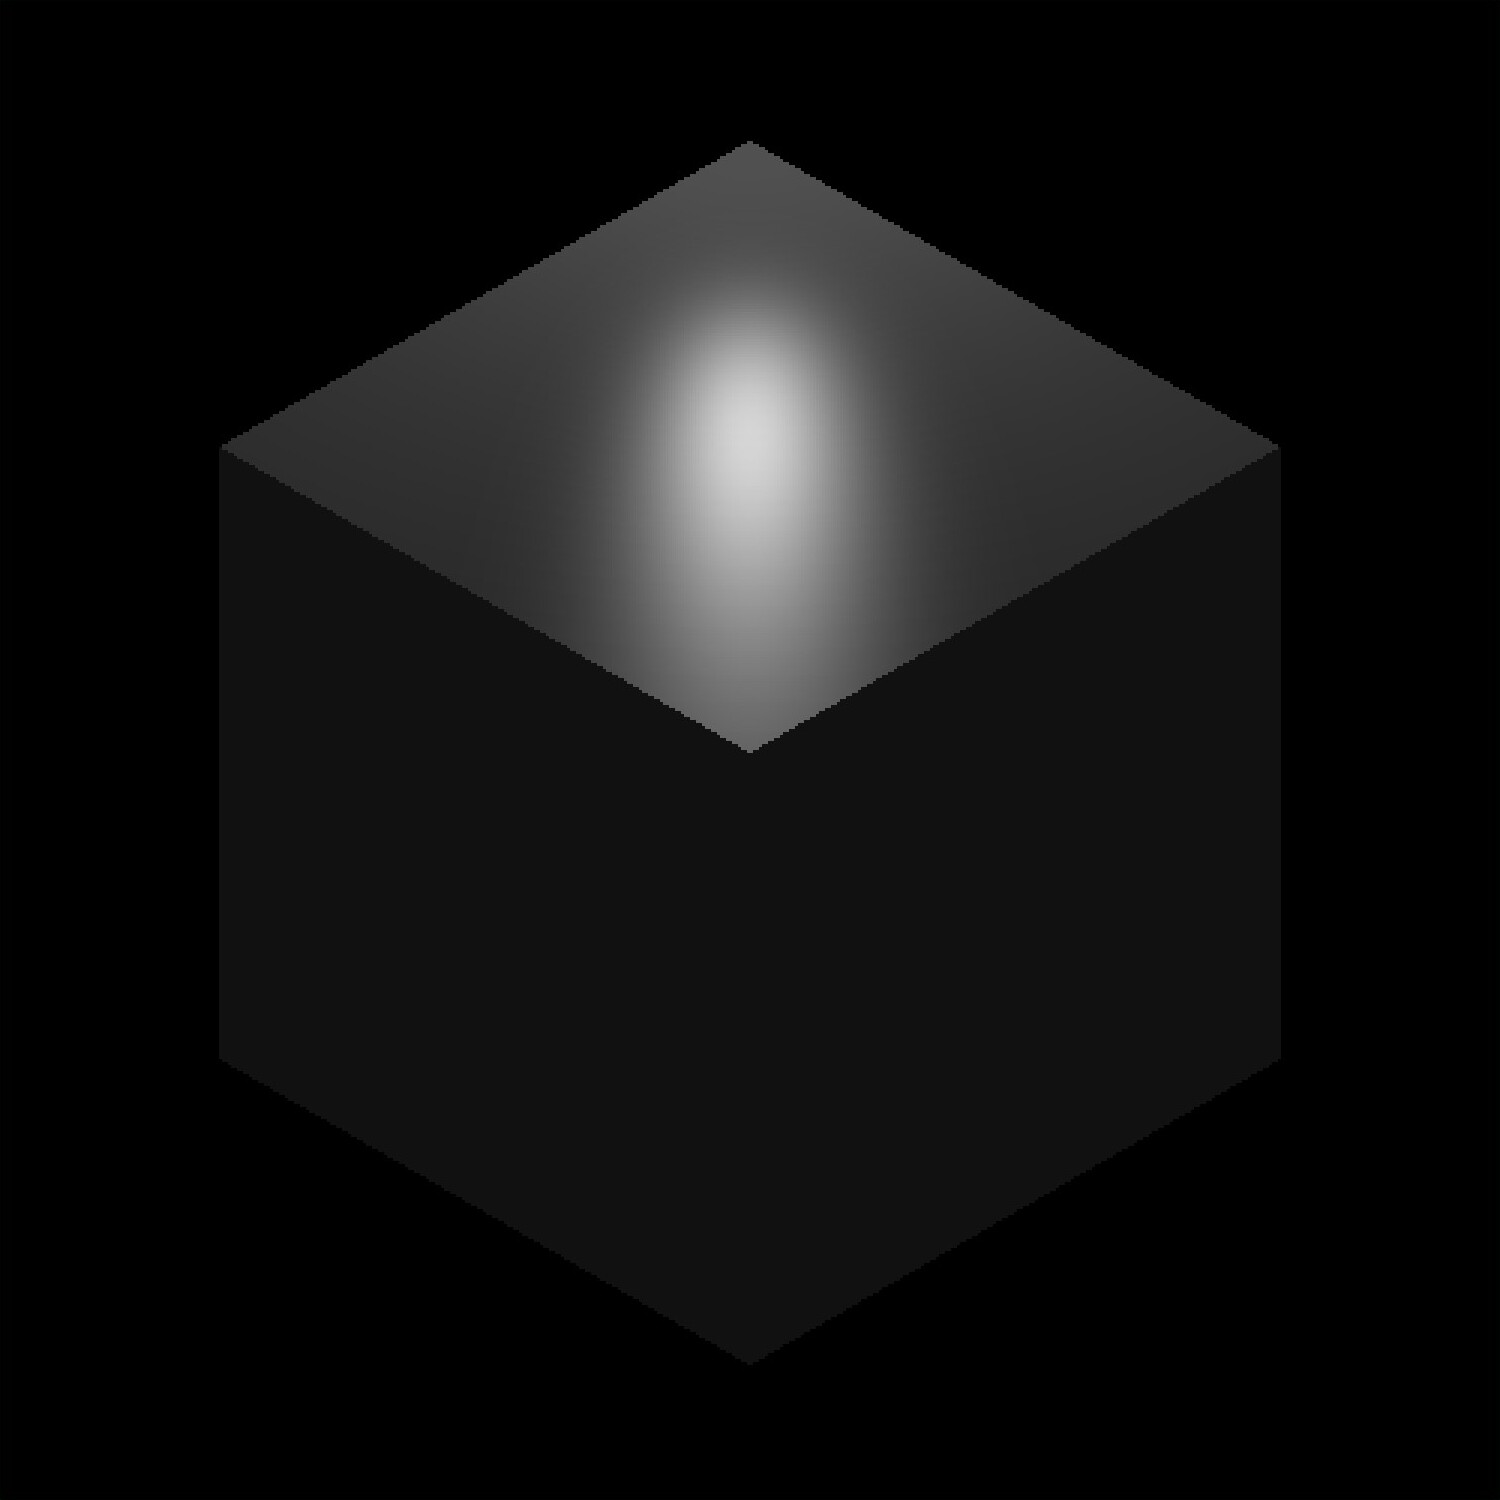
\includegraphics[width=3.8cm]{Cube4.jpg}
%     \end{FigureSub}
%     \hspace{0.5cm}
%     \begin{FigureSub}[$p=1000$;p1000]
%         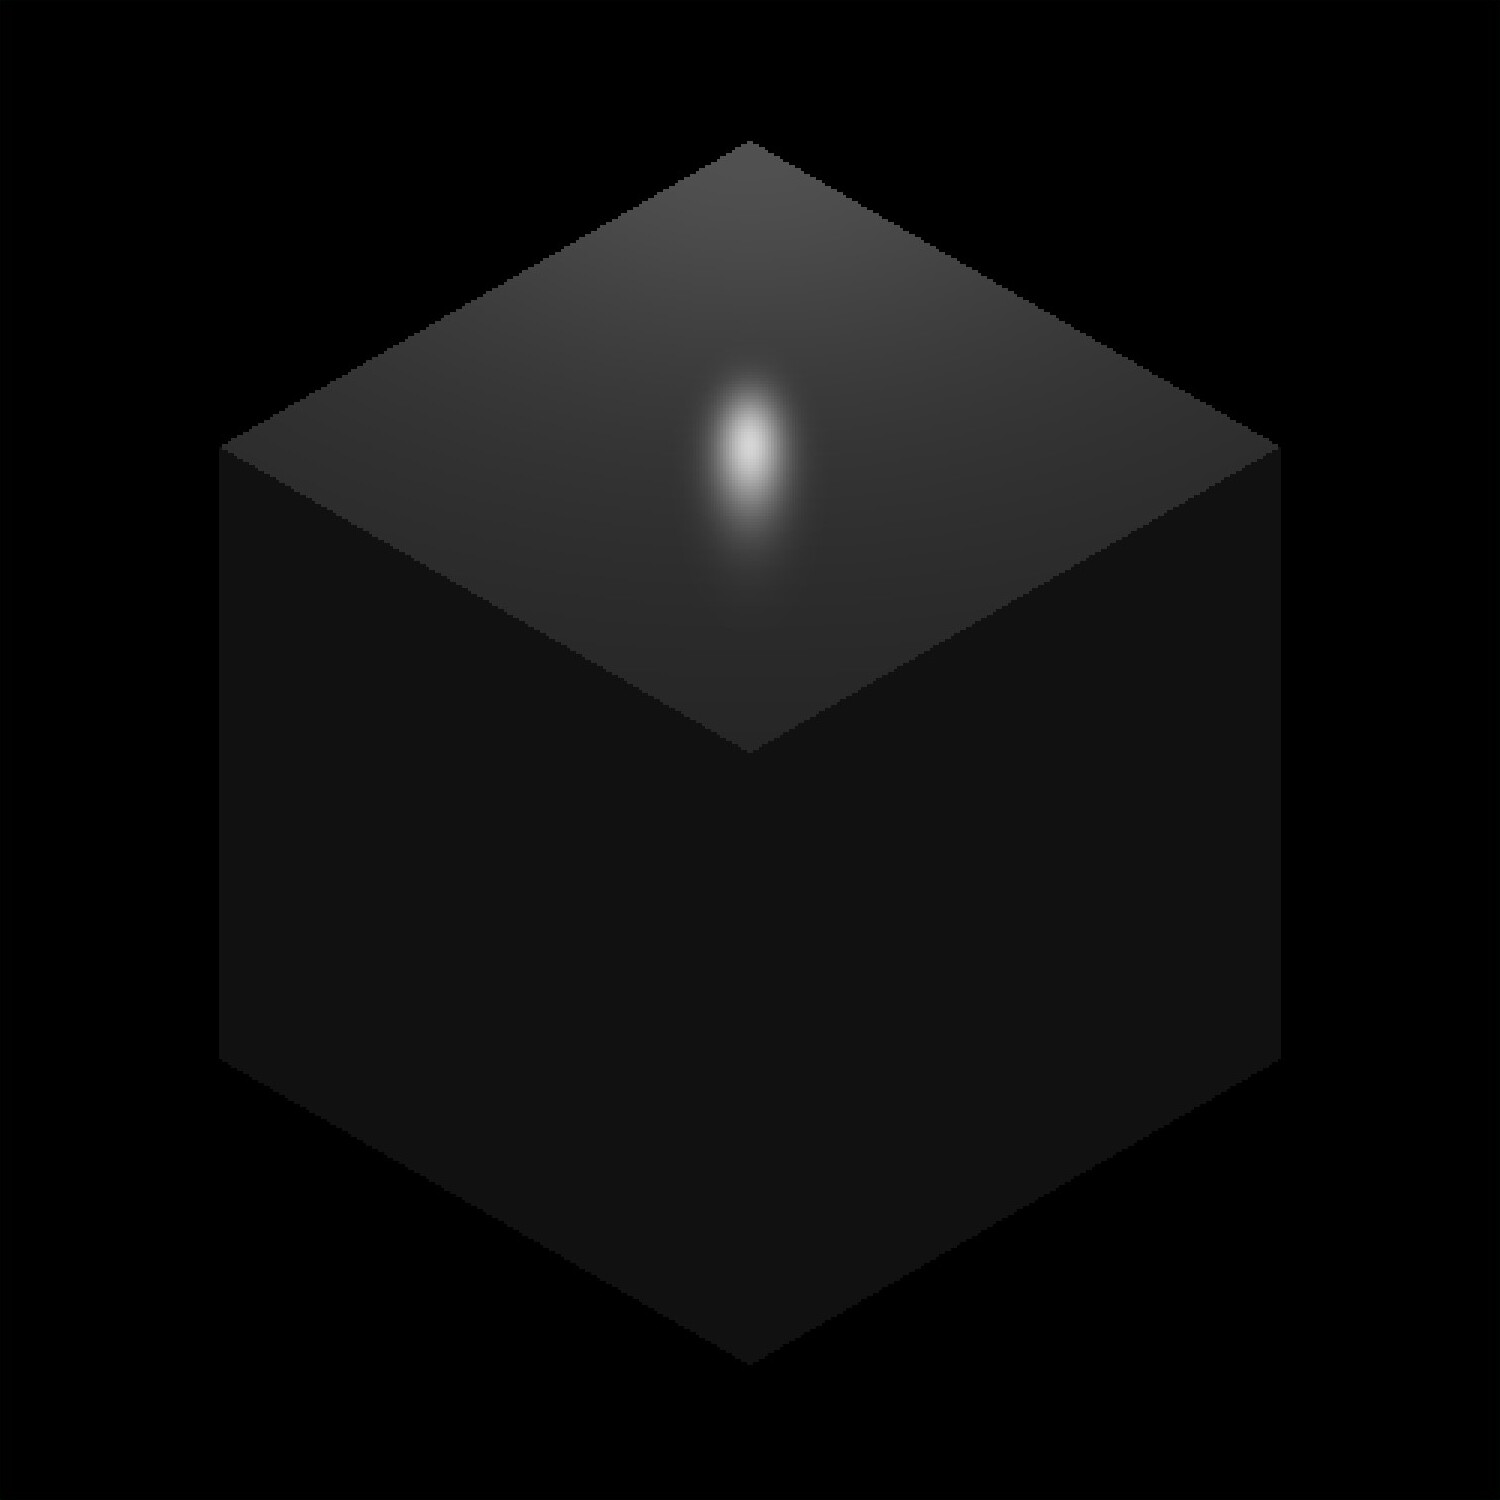
\includegraphics[width=3.8cm]{Cube5.jpg}
%     \end{FigureSub}
% \end{Figure}
% 我们知道,Blinn-Phong着色有效的关键在于,视线需要位于光源反射线上,因此\cref{fig:Lambertian着色和Ambient着色}中的光源布置无法体现Blinn-Phong着色的效果。在\cref{fig:Blinn-Phong着色}中,我们将光源移动至了顶侧,同时降低漫反射颜色$c_d$并增加镜面反射颜色$c_s$以更好凸显高光效果。我们注意到,Blinn-Phong着色使立方体的上侧面表现出了明显的反光,且随着$p$值的增大,高光的光斑就相应越小。

% \chapter{表面着色}
着色(Shading)是指这样一件事,若某条光线追踪的某个物体,那么这条光线对应的像素应该渲染为什么颜色?最朴素的思路是,物体是什么颜色就将像素渲染为什么颜色,这可行但效果肯定不好,试想,这样渲染一个蓝色的球体将得到一个完全是蓝色的圆,毫无立体感。

到底是什么赋予了物体明暗?光源!朴素的说,正对光的面比较亮,侧对光的面比较暗,除此之外,材料有哑光和高光之分。总而言之,着色要研究的就是光源对于物体自身颜色的影响。

\section{Lambertian着色}

Lambertian着色是最简单的模型,其认为,照射至物体表面的光取决于表面和光源的夹角
\begin{itemize}
    \item 若物体表面正对着光源,则表面是完全照亮的。
    \item 若物体表面平行于光源,则表明是完全黑暗的。
\end{itemize}

\begin{Figure}[Lambertian着色]
    \includegraphics[scale=0.8]{build/Chapter05A_01.fig.pdf}
\end{Figure}

如\xref{fig:Lambertian着色}所示,$\vb{n}$是表面的法向,$\vb{l}$是光源的方向,它们都被设定为单位向量。
\begin{BoxFormula}[Lambertian着色]
    Lambertian着色认为
    \begin{Equation}
        c=c_lc_r\max(0,\vb{n}\cdot\vb{l})
    \end{Equation}
\end{BoxFormula}
其中,$c_l$是光源颜色,$c_r$是物体散射颜色,该公式应当对RGB各计算一次以得到RGB每个分量的结果。在\xref{fig:Lambertian着色}中用$\theta$表示$\vb{n},\vb{l}$的夹角,由于$\vb{n},\vb{l}$都是单位矢量,因此$\vb{n}\cdot\vb{l}=\cos\theta$,这符合前面的预期,当$\theta=0$时给出$1$
即最亮,当$\theta=\pm\pi/2$时给出$0$即最暗。然而我们必须要处理的一种情况是当光源位于表面背后,此时$\vb{n}\cdot\vb{l}<0$为负数,这会违背RGB的数值在区间$[0,1]$的要求,而且直观上“不可能比黑更黑”,因此需要将$\vb{n}\cdot\vb{l}$和$0$之间取$\max$函数。

Lambertian着色的一个特点是它与视角无关。这一点我们可以这样理解:Lambertian着色假定物体表面向各方向均匀散射了从光源接收的能量,所以从各个视角看起来都是一样的。
\section{Ambient着色}
Lambertian着色存在的一个问题是,对于物体背对光源部分的表面,将是完全黑暗的,然而这往往和现实不符。物体背光一侧相较迎光一侧肯定要更暗一些,但不可能是完全黑暗的。

Ambient着色改进了这一点,其叠加了一个环境光源$c_a$项
\begin{BoxFormula}[Ambient着色]
    Ambient着色认为
    \begin{Equation}
        c=c_ac_r+c_lc_r\max(0,\vb{n}\cdot\vb{l})
    \end{Equation}
\end{BoxFormula}
Ambient着色可以认为是模拟了现实中由于各个物体的散射使环境中存在的一个各向同性的基础亮度。此外,要指出的是,我们需要确保环境光源和点光源的总和$c_a+c_l<1$,否则会导致RGB的结果溢出$[0,1]$的范围,另外一种可行的方式是当结果高于$1$将其限定在$1$。
\section{Blinn-Phong着色}
现实中许多物体看起来是有光泽的。这是因为,物体表面受到光照时,在散射(Diffuse)机制外还同时存在镜面反射(Specular Reflection)机制。换言之,如果视角在光源产生的入射光对应的反射光方向上,看到的颜色会更亮。Blinn-Phong着色就是在考虑镜面反射的影响。

如\cref{fig:Lambertian着色}所示,$\vb{n}$是表面的法向,$\vb{l},\vb{v}$分别为光源和视线的方向。这里要考察视线方向是否位于光源入射光的反射光上,其实一个等效的做法是,考察$\vb{v},\vb{l}$平分线处的单位矢量$\vb{h}$和表面的法向$\vb{n}$间的夹角$\alpha$有多大?容易证明,我们可以将$\vb{h}$可以表达成以下形式
\begin{Equation}
    \vb{h}=\frac{\vb{v}+\vb{l}}{\norm{\vb{v}+\vb{l}}}
\end{Equation}
因为$\vb{v},\vb{l}$均为单位矢量故$\vb{v}+\vb{l}$必位于两者平分线上,而除以模是为将其也转为单位矢量。

\begin{Figure}[Blinn-Phong着色]
    \includegraphics[scale=0.8]{Chapter05C_01.fig.pdf}
\end{Figure}
基于此,Blinn-Phong着色可以表述为
\begin{BoxFormula}[Blinn-Phong着色]
    Blinn-Phong着色
    \begin{Equation}
        c=c_ac_r+c_lc_r\max(0,\vb{n}\cdot\vb{l})+c_lc_p\max(0,\vb{n}\cdot\vb{h})^p
    \end{Equation}
\end{BoxFormula}
其中,$c_p$是镜面反射颜色,$c_p$和$c_r$不一定要是相同的,但是应当确保$c_p+c_r<1$以保证不会令RGB溢出$[0,1]$的范围。$p$称为Phong指数,它代表了物体表面的光泽度,我们容易看出,$p$越大则镜面反射项$c_lc_p\max(0,\vb{n}\cdot\vb{h})^p$衰减越快,可以这样理解,镜面反射会令视线处于反射光两侧一定角度内出现额外的高光,$p$则会决定高光的范围,$p$越大则高光范围越小。

在\cref{tab:着色过程的符号和表达式整理}中,我们整理了着色中出现的符号和表达式
\begin{Table}[着色过程的符号和表达式整理]!!
    \begin{tblr}{colspec={llZ}}
    颜色或表达式&&说明\\
    $c_r$&&物体表面的散射颜色\\
    $c_p$&&物体表面的反射颜色\\
    $c_l$&&点状光源的颜色\\
    $c_a$&&环境光源的颜色\\
    $c_r+c_p\leq 1$&&物体的颜色和不能超过$1$\\
    $c_l+c_a\leq 1$&&光源的颜色和不能超过$1$\\ \hline
    $c_ac_r$&Ambient&环境光源的散射\\
    $c_lc_r\max(0,\vb{n}\cdot\vb{l})$&Lambertian&点光源的散射\\
    $c_lc_p\max(0,\vb{n}\cdot\vb{h})^{p}$&Blinn-Phong&点光源的反射\\
    \end{tblr}
\end{Table}
\section{着色频率}
在前面三节中,我们讨论了一个点处的颜色应该如何根据光源和视角的方向计算。那么在实践中,对于一个三角面,我们到底要计算多少点的颜色?这就是着色频率,有三个等级

\begin{enumerate}
    \item 平面着色(Flat Shading):面上各点使用同一颜色。
    \item 顶点着色(Gouraud Shading):面上一点的颜色是顶点颜色的插值。
    \item 像素着色(Phong Shading):面上一点的颜色是顶点法向量在该点插值对应的颜色。
\end{enumerate}


这里需要进一步解释的是顶点着色和像素着色,它们都涉及一个问题,什么是顶点处的法向量?这个提法很怪,因为一个三角面只有一个法向量$\vb{n}$。实际上,顶点处的法向量$\vb{n}_a,\vb{n}_b,\vb{n}_c$定义为该顶点连接的所有三角面的法向量的平均值,这样一来,顶点可以均衡考虑临近三角面的方向从而通过后续插值在三角面之间创建比较自然的颜色过渡,而顶点着色和像素着色的差异就在于它们的插值方式略有不同,为此,我们有必要先解释一下三角面上的插值原理。

我们再次写出三角面的参数方程
\begin{Equation}
    \vb{f}=\vb{a}+\beta(\vb{b}-\vb{a})+\gamma(\vb{c}-\vb{a})
\end{Equation}
我们不妨将$\vb{a}$提出
\begin{Equation}
    \vb{f}=(1-\beta-\gamma)\vb{a}+\beta\vb{b}+\gamma\vb{c}
\end{Equation}
引入$\alpha=1-\beta-\gamma$
\begin{Equation}
    \vb{f}=\alpha\vb{a}+\beta\vb{b}+\gamma\vb{c}
\end{Equation}
三角面上任意一点都可以由$(\alpha,\beta,\gamma)$表示,这称为重心坐标(Barycentric Coordinate)。而如果三个顶点处有某个量$x_a,x_b,x_c$,那么$(\alpha,\beta,\gamma)$处的$x$就可由$x=\alpha x_a+\beta x_b+\gamma x_c$插值。

顶点着色的意思是,根据$\vb{n}_a,\vb{n}_b,\vb{n}_c$先算出顶点处的颜色$c_a,c_b,c_c$,随后插值出颜色
\begin{Equation}
    c=\alpha c_a+\beta c_b+\gamma c_c
\end{Equation}
像素着色的意思是,根据$\vb{n}_a,\vb{n}_b,\vb{n}_c$先插值出待计算点处的法向量$\vb{n}$,随后再通过该点处的法向量$\vb{n}$计算出相应的颜色,假如记颜色和法向量间的函数关系为$f$,则有
\begin{Equation}
    c=f(\alpha \vb{n}_a+\beta \vb{n}_b+\gamma \vb{n}_c)
\end{Equation}
简而言之,顶点着色插值对象为颜色,像素着色插值对象为法向量。像素着色的精度要优于顶点着色,尽管似乎只是颜色计算和插值计算互换了一下顺序,但这样一来,像素着色能赋予三角面上每个点均匀变化的法向量,这对于对法向量极为敏感的Blinn-Phong着色模型很重要。


% \begin{enumerate}
%     \item 频率为三角面(Flat Shading),三角面上各点使用同一颜色。
%     \item 频率为顶点(Gouraud Shading),三角面上一点的颜色是顶点颜色的插值。
%     \item 频率为像素(Phong Shading),三角面上一点的颜色是顶点法向量在该点插值对应的颜色。
% \end{enumerate}
\chapter{线性代数}
% 渲染分为图像顺序渲染和物体顺序渲染两种,在\xref{chap:光线追踪}中,我们已经介绍了图像顺序渲染的典型算法光线追踪。在接下来的几章,我们将转向物体顺序渲染,主要分为两个部分
% \begin{itemize}
%     \item 视角变换(Viewing Transformation),研究如何将三维空间的坐标变化到二维平面上。
%     \item 光栅化(Raterization),研究如何将二维平面上的图形转换为离散的像素点。
% \end{itemize}

在本章,我们将研究视角变换部分的基础数学,即如何用矩阵实现各种变换?首先我们将从二维出发介绍四种基本的矩阵变换,随后我们会介绍矩阵的特征值分解和奇异值分解,进而将矩阵变换推广至三维并解决三维中常用的法向量在矩阵变换中遇到的特殊问题,最后我们会研究如何通过齐次坐标优雅的表示仿射变换,并以此为基础,介绍坐标系变换的表示方法。

\section{矩阵变换}


\section{矩阵变换的分解}
本节将研究这样一个问题,对于一般的变换矩阵$\vb{A}$,如何将其拆分为若干基本变换的叠加?

在开始前,有必要说明一下几种特殊矩阵的定义。
\begin{BoxDefinition}[对角矩阵]
    对角矩阵(Diagonal Matrix)是指仅具有对角元素的矩阵
    \begin{Equation}
        \vb{A}=\te{diag}(a_1,a_2)=\begin{pmatrix}
            a_1&0\\
            0&a_2\\
        \end{pmatrix}
    \end{Equation}
\end{BoxDefinition}

\begin{BoxDefinition}[对称矩阵]
    对称矩阵(Symmetric Matrix)是指转置与自身相等的矩阵
    \begin{Equation}
        \vb{A}=\vb{A}^T
    \end{Equation}
\end{BoxDefinition}
显然,对角矩阵一定是一个对称矩阵。

\begin{BoxDefinition}[正交矩阵]
    正交矩阵(Orthogonal Matrix)是指转置与自身的积为单位阵的矩阵
    \begin{Equation}
        \vb{A}^T\vb{A}=\vb{I}
    \end{Equation}
\end{BoxDefinition}
这里有一个很重要的性质:若一个矩阵$\vb{A}$的列是由一组相互正交的单位向量组成,那么该矩阵一定是一个正交矩阵!试想,对于$\vb{A}^T\vb{A}$的乘积结果,其对角元素是一个单位向量与其自身的点积,因而是$1$,其非对角元素是两个正交向量的点积,因而是$0$,这样就有$\vb{A}^T\vb{A}=\vb{I}$。

\subsection{特征值分解}
在继续介绍特征值分解前,我们有必要先回顾一下特征值和特征向量的概念。

对于一个矩阵$\vb{A}$,若能找到向量$\vb{a}$和数$\lambda$使
\begin{Equation}
    \vb{A}\vb{a}=\lambda\vb{a}
\end{Equation}
那么$\vb{a},\lambda$就称为$\vb{A}$的一组特征向量(Eigen Vector)和特征值(Eigen Value)。换言之,若矩阵作用在一个向量上却只会令这个向量伸长或压缩,那么这个向量就是矩阵的特征向量。

很重要的问题是如何寻找特征向量和特征值?我们可以先加入一个$\vb{I}$\setpeq{求解特征向量和特征值}
\begin{Equation}&[1]
    \vb{A}\vb{a}=\lambda\vb{I}\vb{a}
\end{Equation}
移项至左侧
\begin{Equation}&[2]
    \vb{A}\vb{a}-\lambda\vb{I}\vb{a}=0
\end{Equation}
提出矩阵
\begin{Equation}&[3]
    (\vb{A}-\lambda\vb{I})\vb{a}=0
\end{Equation}
该方程成立唯一的条件是$\vb{A}-\lambda\vb{I}$是一个奇异阵,换言之,行列式为$0$。假设$\vb{A}$是$2\times 2$的
\begin{Equation}&[4]
    \begin{vmatrix}
        a_{11}-\lambda&a_{12}\\
        a_{21}&a_{22}-\lambda\\
    \end{vmatrix}=0
\end{Equation}
即
\begin{Equation}&[5]
    \lambda^2-(a_{11}+a_{22})\lambda+(a_{11}a_{22}-a_{12}a_{21})=0
\end{Equation}
这是一个二次方程,故可以解出两个特征值$\lambda$。事实上,对于一个$n\times n$的矩阵,其具有$n$个特征值。由于四次以上的方程无系解析解,故对于$n>4$的矩阵,其特征值只有数值解。


而对于某个已经求出的特征值$\lambda$,也很容易确定对应的特征向量$\vb{a}=(x,y)$,考虑\xrefpeq{3}
\begin{Equation}
    \begin{pmatrix}
        a_{11}-\lambda&a_{12}\\
        a_{21}&a_{22}-\lambda\\
    \end{pmatrix}
    \begin{pmatrix}
        x\\
        y\\
    \end{pmatrix}=
    \begin{pmatrix}
        0\\
        0\\
    \end{pmatrix}
\end{Equation}
这是一个齐次方程,有无穷多组非零$(x,y)$是方程的解,注意到
\begin{Equation}
    (a_{11}-\lambda)x+a_{12}y=a_{21}x+(a_{22}-\lambda)y
\end{Equation}
整理得到
\begin{Equation}
    (a_{11}-a_{21}-\lambda)x=(a_{22}-a_{12}-\lambda)y
\end{Equation}
因此,只要$x,y$符合下面的比例,那它就是$\lambda$对应的特征向量
\begin{Equation}
    \frac{y}{x}=\frac{a_{11}-a_{21}-\lambda}{a_{22}-a_{12}-\lambda}
\end{Equation}
这一点从特征值的定义$\vb{A}\vb{a}=\lambda \vb{a}$上看也很合理:若$\vb{a}$是特征向量,那么$\vb{a}$的任意倍也都是特征向量,毕竟这只不过是在方程两端同乘了一个相同的系数罢了。但通常,我们会选择那个长度为$1$的那个单位特征向量。除此之外,可以证明一个矩阵的特征向量是两两相互正交的。\goodbreak

任何一个矩阵都具有特征向量和特征值,然而,若矩阵是满足对称矩阵,则矩阵自身可以直接用其特征向量和特征值表示出来,这就是所谓的特征值分解!它的具体形式如下
\begin{BoxFormula}[特征值分解]
    特征值分解(Eigen Value Decomposition, EVD)是指,对于对称矩阵$\vb{A}$,有
    \begin{Equation}
        \vb{A}=\vb{R}\vb{S}\vb{R}^T
    \end{Equation}
    矩阵$\vb{R}$是一个正交矩阵,由特征向量$\vb{r}_1,\vb{r}_2$构成
    \begin{Equation}
        \vb{R}=\qty(\vb{r}_1,\vb{r}_2)
    \end{Equation}
    矩阵$\vb{S}$是一个对角矩阵,由特征值$\lambda_1,\lambda_2$构成
    \begin{Equation}
        \vb{S}=\te{diag}(\lambda_1,\lambda_2)
    \end{Equation}
\end{BoxFormula}

现在我们来解读结果,不过再次之前,我们先要将特殊矩阵和矩阵变换联系起来
\begin{itemize}
    \item 对角矩阵$\vb{S}=\te{diag}(\lambda_1,\lambda_2)$对应缩放变换,其中$\lambda_1,\lambda_2$代表沿$\vb{x},\vb{y}$的缩放比。
    \item 正交矩阵$\vb{R}=(\vb{r}_1,\vb{r}_2)$对应旋转变换,其代表$\vb{x},\vb{y}$旋转至$\vb{r}_1,\vb{r}_2$方向,$\vb{R}^T$则相反。
\end{itemize}

特征值分解可以视为这样三步变换
\begin{enumerate}
    \item 旋转,矩阵$\vb{R}^T$作用,代表图形由$\vb{r}_1,\vb{r}_2$方向分别旋转至$\vb{x},\vb{y}$方向。
    \item 缩放,矩阵\hspace{0.45em}$\vb{S}$\hspace{0.45em}作用,代表图形沿$\vb{x},\vb{y}$方向分别缩放$\lambda_1,\lambda_2$倍。
    \item 旋转,矩阵$\vb{R}$作用,代表图形由$\vb{x},\vb{y}$方向分别旋转至$\vb{r}_1,\vb{r}_2$方向。
\end{enumerate}
特征值分解告诉我们,任何对称矩阵代表的变换,本质上都可以视为由“旋转--缩放--旋转”这样三步基本变换的组合变换。更进一步的说,由于缩放沿$\vb{x},\vb{y}$进行,且缩放前后的旋转分别是从特征向量方向旋转至$\vb{x},\vb{y}$再旋转回去,因此,对称矩阵的变换的效果其实就是在特征向量$\vb{r}_1,\vb{r}_2$的方向上分别进行特征值$\lambda_1,\lambda_2$倍的缩放!这是一个非常深刻且直观的几何理解。

\subsection{奇异值分解}
奇异值和奇异值分解的想法是从特征值分解延拓出来的。特征值分解存在一个明显的缺陷,即只有对角矩阵才能适用。奇异值分解期望将任何矩阵都拆分为“旋转--缩放--旋转”的形式,不过势必要做出一些让步,需要将$\vb{A}=\vb{R}\vb{S}\vb{R}^T$需改写为$\vb{A}=\vb{U}\vb{S}\vb{V}^T$,即首尾两个正交矩阵不再是同一个。将左侧$\vb{U}=(\vb{u}_1,\vb{u}_2)$和右侧$\vb{v}=(\vb{v}_1,\vb{v}_2)$中的向量分别称为左奇异向量和右奇异向量(Singular Vector),同时,将$\vb{S}=\te{diag}(\sigma_1,\sigma_2)$中的数称为奇异值(Singular Value)。

\begin{BoxFormula}[奇异值分解]
    奇异值分解(Singular Value Decomposition, SVD)是指,对于矩阵$\vb{A}$,有
    \begin{Equation}
        \vb{A}=\vb{U}\vb{S}\vb{V}^T
    \end{Equation}
    矩阵$\vb{U},\vb{V}$是正交矩阵,由左奇异向量$\vb{u}_1,\vb{u}_2$和右奇异向量$\vb{v}_1,\vb{v}_2$构成
    \begin{Equation}
        \vb{U}=\qty(\vb{u}_1,\vb{u}_2)\qquad
        \vb{V}=\qty(\vb{v}_1,\vb{v}_2)
    \end{Equation}
    矩阵$\vb{S}$是一个对角矩阵,由特征值$\sigma_1,\sigma_2$构成
    \begin{Equation}
        \vb{S}=\te{diag}(\sigma_1,\sigma_2)
    \end{Equation}
\end{BoxFormula}

奇异值分解可以视为这样三步变换
\begin{itemize}
    \item 旋转,矩阵$\vb{V}^T$作用,代表图形由$\vb{v}_1,\vb{v}_2$方向分别旋转至$\vb{x},\vb{y}$方向。
    \item 缩放,矩阵\hspace{0.45em}$\vb{S}$\hspace{0.45em}作用,代表图形沿$\vb{x},\vb{y}$方向分别缩放$\sigma_1,\sigma_2$倍。
    \item 旋转,矩阵$\vb{U}$作用,代表图形由$\vb{x},\vb{y}$方向分别旋转至$\vb{u}_1,\vb{u}_2$方向。
\end{itemize}

奇异值分解和特征值分解能如何联系在一起呢?考虑以下矩阵
\begin{Equation}
    \vb{M}=\vb{A}\vb{A}^T
\end{Equation}
代入$\vb{A}=\vb{U}\vb{S}\vb{V}^T$
\begin{Equation}
    \vb{M}=(\vb{U}\vb{S}\vb{V}^T)(\vb{U}\vb{S}\vb{V}^T)^T
\end{Equation}
若干矩阵乘积的转置,等于每个矩阵转置的逆序乘积
\begin{Equation}
    \vb{M}=(\vb{U}\vb{S}\vb{V}^T)(\vb{V}\vb{S}^T\vb{U}^T)
\end{Equation}
由于$\vb{S}$是对角矩阵,故$\vb{S}^T=\vb{S}$
\begin{Equation}
    \vb{M}=(\vb{U}\vb{S}\vb{V}^T)(\vb{V}\vb{S}\vb{U}^T)
\end{Equation}
应用矩阵乘法的分配律
\begin{Equation}
    \vb{M}=\vb{U}\vb{S}(\vb{V}^T\vb{V})\vb{S}\vb{U}^T
\end{Equation}
由于$\vb{V}$是对角矩阵,故$\vb{V}^T\vb{V}=\vb{I}$
\begin{Equation}
    \vb{M}=\vb{U}\vb{S}^2\vb{U}^T
\end{Equation}
这意味着$\vb{M}=\vb{A}^T\vb{A}$必然可以做特征值分解!且此时,特征向量是$\vb{A}$的左奇异向量,特征值是$\vb{A}$的奇异值的平方,因为$\vb{S}^2=\te{diag}(\sigma_1^2,\sigma_2^2)$。由此可见,通过这种方式,奇异值的计算可以转换为特征值的计算。并且,$\vb{A}^T\vb{A}=\vb{U}\vb{S}^2\vb{U}^T$给出$\vb{U}$,类似的,$\vb{A}\vb{A}^T=\vb{V}\vb{S}^2\vb{V}^T$给出$\vb{V}$。
\section{三维中的矩阵变换}
三维中的矩阵变换和二维中的情形类似,我们将相关矩阵列举如下。
\begin{BoxDefinition}[三维缩放变换]
    三维缩放变换定义为
    \begin{Equation}
        \te{scale}(s_x,s_y,s_z)=
        \begin{pmatrix}
            s_x&0&0\\
            0&s_y&0\\
            0&0&s_z\\
        \end{pmatrix}
    \end{Equation}
\end{BoxDefinition}

三维中的剪切有沿$x,y,z$三个方向的,每一种剪切都涉及另外两个方向的剪切系数。
\begin{BoxDefinition}[三维剪切变换]
    三维中,沿$x$方向的剪切变换定义为
    \begin{Equation}
        \te{shear}_x(d_y,d_z)=
        \begin{pmatrix}
            1&d_y&d_z\\
            0&1&0\\
            0&0&1\\
        \end{pmatrix}
    \end{Equation}
    三维中,沿$y$方向的剪切变换定义为
    \begin{Equation}
        \te{shear}_y(d_z,d_x)=
        \begin{pmatrix}
            1&0&0\\
            d_x&1&d_z\\
            0&0&1\\
        \end{pmatrix}
    \end{Equation}
    三维中,沿$z$方向的剪切变换定义为
    \begin{Equation}
        \te{shear}_z(d_x,d_y)=
        \begin{pmatrix}
            1&0&0\\
            0&1&0\\
            d_x&d_y&1\\
        \end{pmatrix}
    \end{Equation}
\end{BoxDefinition}

三维中的旋转有一些不一样。我们知道,旋转是围绕一根轴在一个面内进行的,二维的旋转只能在二维平面上进行,故只有一种旋转矩阵,但在三维下旋转则可以绕$x,y,z$轴旋转。
\begin{BoxDefinition}[三维旋转变换]*
    三维中,绕$x$轴的旋转变换定义为
    \begin{Equation}
        \te{rotate}_x(\phi)=
        \begin{pmatrix}
            1&0&0\\
            0&\cos\phi&-\sin\phi\\
            0&\sin\phi&\cos\phi\\
        \end{pmatrix}
    \end{Equation}
    三维中,绕$y$轴的旋转变换定义为
    \begin{Equation}
        \te{rotate}_y(\phi)=
        \begin{pmatrix}
            \cos\phi&0&\sin\phi\\
            0&1&0\\
            -\sin\phi&0&\cos\phi\\
        \end{pmatrix}
    \end{Equation}
    三维中,绕$z$轴的旋转变换定义为
    \begin{Equation}
        \te{rotate}_z(\phi)=
        \begin{pmatrix}
            \cos\phi&-\sin\phi&0\\
            \sin\phi&\cos\phi&0\\
            0&0&1\\
        \end{pmatrix}
    \end{Equation}
\end{BoxDefinition}

三维中的反射有翻转$x,y,z$轴三种,但下标记录的是以什么面进行对称。

\begin{BoxDefinition}[三维翻转变换]*
    三维中,以$y,z$平面为对称面(翻转$x$轴)的反射变换定义为
    \begin{Equation}
        \te{reflect}_{yz}=
        \begin{pmatrix}
            -1&0&0\\
            0&1&0\\
            0&0&1\\
        \end{pmatrix}
    \end{Equation}
    三维中,以$z,x$平面为对称面(翻转$y$轴)的反射变换定义为
    \begin{Equation}
        \te{reflect}_{zx}=
        \begin{pmatrix}
            1&0&0\\
            0&-1&0\\
            0&0&1\\
        \end{pmatrix}
    \end{Equation}
    三维中,以$x,y$平面为对称面(翻转$z$轴)的反射变换定义为
    \begin{Equation}
        \te{reflect}_{xy}=
        \begin{pmatrix}
            1&0&0\\
            0&1&0\\
            0&0&-1\\
        \end{pmatrix}
    \end{Equation}
\end{BoxDefinition}

\subsection{法向量变换}

在三维空间中,我们经常会用法向量表示一个面的方向,然而,法向量进行变换后往往不再是法向量。\cref{fig:法向量在三维变换中的问题}展示了这一问题,矩形经过变换矩阵$\vb{M}$的剪切变换后,法向量$\vb{n}$顺着剪切变为了斜向上的$\vb{M}\vb{n}$,但其实$\vb{M}\vb{n}$并不垂直于平面,此时,正确的法向量应是图中标出的$\vb{N}\vb{n}$。

这就告诉我们,当图形通过矩阵$\vb{M}$变换时,法向量若也通过矩阵$\vb{M}$变换将得到不正确的结果,法向量需要另外一个不同的矩阵$\vb{N}$矩形进行变换。故现在的问题是怎么由$\vb{M}$求出$\vb{N}$?

\begin{Figure}[法向量在三维变换中的问题]
    \figuresub[变换前;变换前--法向量在三维变换中的问题]{\includegraphics[scale=0.8]{Chapter06C_01.fig.pdf}}{0.48}
    \figuresub[变换后;变换后--法向量在三维变换中的问题]{\includegraphics[scale=0.8]{Chapter06C_02.fig.pdf}}{0.48}
\end{Figure}
首先,可以确定的是变换前法向量$\vb{n}$一定垂直于切向量$\vb{t}$
\begin{Equation}[法向量变换1]
    \vb{n}^T\vb{t}=0
\end{Equation}

我们将变换后的向量用$\vb{n}_N=\vb{N}\vb{n},~\vb{n}_M=\vb{M}\vb{n},~\vb{t}_M=\vb{M}\vb{t}$表示,我们要找到$\vb{N}$使下式成立
\begin{Equation}[法向量变换2]
    \vb{n}_N^T\vb{t}_M=0
\end{Equation}
我们可以在\cref{eq:法向量变换1}做一些变形,利用$\vb{M}^{-1}\vb{M}=\vb{I}$
\begin{Equation}
    \vb{n}^T\vb{t}=\vb{n}^T\vb{I}\vb{t}=\vb{n}^T\vb{M}^{-1}\vb{M}\vb{t}=0
\end{Equation}
应用矩阵乘法的分配律
\begin{Equation}
    (\vb{n}^T\vb{M}^{-1})(\vb{M}\vb{t})=0
\end{Equation}
注意到$\vb{M}\vb{t}$就是$\vb{t}_M$
\begin{Equation}
    (\vb{n}^T\vb{M}^{-1})\vb{t}_M=0
\end{Equation}
比照\cref{eq:法向量变换2},即得
\begin{Equation}
    \vb{n}_N^T=\vb{n}^T\vb{M}^{-1}
\end{Equation}
两边转置
\begin{Equation}
    \vb{n}_N=(\vb{M}^{-1})^T\vb{n}
\end{Equation}

由此可见应有$\vb{N}=(\vb{M}^{-1})^T$,即适用法向量变换的$\vb{N}$是$\vb{M}$的逆矩阵的转置。
\begin{BoxFormula}[法向量变换]
    法向量的变换矩阵$\vb{N}$为
    \begin{Equation}
        \vb{N}=(\vb{M}^{-1})^T
    \end{Equation}
\end{BoxFormula}

我们可以证明,这里$\vb{N}$可以写为
\begin{Equation}
    \vb{N}=
    \begin{pmatrix}
        m_{11}^c&m_{12}^c&m_{13}^c\\
        m_{21}^c&m_{22}^c&m_{23}^c\\
        m_{31}^c&m_{32}^c&m_{33}^c\\    
    \end{pmatrix}
\end{Equation}
其中$m_{ij}^c$代表$\vb{M}$在$m_{ij}$处的代数余子式,完整展开的结果是
\begin{Equation}
    \vb{N}=
    \begin{pmatrix}
        m_{22}m_{33}-m_{23}m_{32}&
        m_{23}m_{31}-m_{21}m_{33}&
        m_{21}m_{32}-m_{22}m_{31}\\
        m_{13}m_{32}-m_{12}m_{33}&
        m_{11}m_{33}-m_{13}m_{31}&
        m_{12}m_{31}-m_{11}m_{32}\\
        m_{12}m_{23}-m_{13}m_{22}&
        m_{13}m_{21}-m_{11}m_{23}&
        m_{11}m_{22}-m_{12}m_{21}\\
    \end{pmatrix}
\end{Equation}
实际上,严格来说上式还要再除以$\vb{M}$的行列式才是真正的$\vb{N}=(\vb{M}^{-1})^T$,但由于法向量并不关心长度(反正最终都要对$\vb{N}\vb{n}$归一化),计算$\vb{N}=(\vb{M}^{-1})^T$时省略除行列式不影响结果。
\section{仿射变换与平移}
通过前面几节,我们已经很清楚的认识到,在三维空间中的一个线性变换可以写成
\begin{Equation}
    \begin{pmatrix}
        x'\\
        y'\\
        z'\\
    \end{pmatrix}=
    \begin{pmatrix}
        m_{11}&m_{12}&m_{13}\\
        m_{21}&m_{22}&m_{23}\\
        m_{31}&m_{32}&m_{33}
    \end{pmatrix}
    \begin{pmatrix}
        x\\
        y\\
        z\\
    \end{pmatrix}
\end{Equation}
我们可以展开来写
\begin{Gather}
    x'=m_{11}x+m_{12}y+m_{13}z\\
    y'=m_{21}x+m_{22}y+m_{23}z\\
    z'=m_{31}x+m_{32}y+m_{33}z
\end{Gather}
我们通过不同的系数可以用上式表示缩放、剪切、旋转、反射等各种变换,但是,却无法表示最简单的平移!换言之,所有变换都是以$(0,0,0)$为中心进行的。若要考虑平移,则需有
\begin{Gather}
    x'=m_{11}x+m_{12}y+m_{13}z+x_t\\
    y'=m_{21}x+m_{22}y+m_{23}z+y_t\\
    z'=m_{31}x+m_{32}y+m_{33}z+z_t
\end{Gather}
诚然,我们可以将$\vb{r}'=\vb{M}\vb{r}$改写为$\vb{r}'=\vb{M}\vb{r}+\vb{r}_t$来单独处理平移的影响。然而这样做不够优雅,我们希望将平移也囊括在矩阵乘法内,这该怎么做呢?有一个极为巧妙的方法是引入齐次坐标(Homogeneous Coordinates)的概念,简单来说,它为每个向量多加了一个维度
\begin{Equation}
    \begin{pmatrix}
        x\\
        y\\
        z\\
        1\\
    \end{pmatrix}\qquad
    \begin{pmatrix}
        x\\
        y\\
        z\\
        0\\
    \end{pmatrix}
\end{Equation}
这个新增的第四维度的元素可以被填充为$0$和$1$
\begin{itemize}
    \item 添加$1$,代表该向量是一个“位矢”,(绝对位置、方位)。
    \item 添加$0$,代表该向量是一个“位移”,(相对位置、方向)。
\end{itemize}
这个设计是很合理且自然的,试想,两个“位置”的差就自然是一个“位矢”
\begin{Equation}
    \begin{pmatrix}
        x_1\\
        y_1\\
        z_1\\
        1\\
    \end{pmatrix}-
    \begin{pmatrix}
        x_2\\
        y_2\\
        z_2\\
        1\\
    \end{pmatrix}=
    \begin{pmatrix}
        x_1-x_2\\
        y_1-y_2\\
        z_1-z_2\\
        0\\
    \end{pmatrix}
\end{Equation}
而有了齐次坐标的定义后,平移就可以通过矩阵乘一并处理了
\begin{Equation}
    \begin{pmatrix}
        x'\\
        y'\\
        z'\\
        1\\
    \end{pmatrix}=
    \begin{pmatrix}
        m_{11}&m_{12}&m_{13}&x_t\\
        m_{21}&m_{22}&m_{23}&y_t\\
        m_{31}&m_{32}&m_{33}&z_t\\
        0&0&0&1\\
    \end{pmatrix}
    \begin{pmatrix}
        x\\
        y\\
        z\\
        1\\
    \end{pmatrix}
\end{Equation}

要注意,这里是“\textbf{先做线性变换,后做平移变换}”,若拆分开来写,则先作用的在后
\begin{Equation}
    \begin{pmatrix}
        x'\\
        y'\\
        z'\\
        1\\
    \end{pmatrix}=
    \begin{pmatrix}
        1&0&0&x_t\\
        0&1&0&y_t\\
        0&0&1&z_t\\
        0&0&0&1\\
    \end{pmatrix}
    \begin{pmatrix}
        m_{11}&m_{12}&m_{13}&0\\
        m_{21}&m_{22}&m_{23}&0\\
        m_{31}&m_{32}&m_{33}&0\\
        0&0&0&1\\
    \end{pmatrix}
    \begin{pmatrix}
        x\\
        y\\
        z\\
        1\\
    \end{pmatrix}
\end{Equation}

这种包含了平移变换的线性变换称为仿射变换(Affine Transformation)。这里可以看出齐次坐标最妙的一点,它不仅解决了平移,而且,倘若参与仿射变换的齐次坐标中的第四维度元素是$0$而不是$1$,即代表参与变换的是一个“位移”而不是“位矢”,则$x_t,y_t,z_t$代表的平移不会作用,且变换后该位置仍为$0$。这是合理的,因为相对距离不会在整体平移中发生变化!

\begin{BoxDefinition}[仿射变换]
    仿射变换矩阵为
    \begin{Equation}
        \vb{M}=
        \begin{pmatrix}
            m_{11}&m_{12}&m_{13}&x_t\\
            m_{21}&m_{22}&m_{23}&y_t\\
            m_{31}&m_{32}&m_{33}&z_t\\
            0&0&0&1\\
        \end{pmatrix}
    \end{Equation}
\end{BoxDefinition}

仿射变换和齐次坐标极大的简化了变换的表示,之后我们还会进一步拓展齐次坐标的用途。

\section{坐标系变换}
在这一节,我们讨论有关坐标系变换的问题,如\cref{fig:坐标系变换}所示。我们知道,在三维空间下的坐标系可以由其原点和三个基矢表征,$xyz$坐标系包含$\vb{o},\vb{x},\vb{y},\vb{z}$,$uvw$坐标系包含$\vb{e},\vb{u},\vb{v},\vb{w}$。假设空间中有一个点$\vb{p}$,在两个坐标系下的坐标分别是$(x_p,y_p,z_p)$和$(u_p,v_p,w_p)$,我们应该如何在两者间转换?首先,从$uvw$系到$xyz$系是很容易的,这基本上就是一些加法
\begin{Equation}
    \vb{p}=\vb{e}+u_p\vb{u}+v_p\vb{v}+w_p\vb{w}
\end{Equation}

我们可以用矩阵的方式来表示
\begin{Equation}[坐标系变换1]
    \begin{pmatrix}
        x_p\\
        y_p\\
        z_p\\
        1
    \end{pmatrix}=
    \begin{pmatrix}
        x_u&x_v&x_w&x_e\\
        y_u&y_v&y_w&y_e\\
        z_u&z_v&z_w&z_e\\
        0&0&0&1\\
    \end{pmatrix}
    \begin{pmatrix}
        u_p\\
        v_p\\
        w_p\\
        1
    \end{pmatrix}
\end{Equation}

我们可以更紧凑的写为
\begin{Equation}[坐标系变换2]
    \vb{p}_{xyz}=\begin{pmatrix}
        \vb{u}&\vb{v}&\vb{w}&\vb{e}\\
        0&0&0&1\\
    \end{pmatrix}
    \vb{p}_{uvw}
\end{Equation}

现在的问题是,通常遇到的坐标变换问题并不是这个方向的。我们往往是期望从$xyz$坐标系变换到$uvw$坐标系,该过程是\cref{eq:坐标系变换2}过程的逆过程,因此变换矩阵要变为对应的逆矩阵
\begin{Equation}[坐标系变换3]
    \vb{p}_{uvw}=\begin{pmatrix}
        \vb{u}&\vb{v}&\vb{w}&\vb{e}\\
        0&0&0&1\\
    \end{pmatrix}^{-1}
    \vb{p}_{xyz}
\end{Equation}

\begin{Figure}[坐标系变换]
    \includegraphics[scale=0.8]{Chapter06E_01.fig.pdf}
\end{Figure}

然而一般矩阵求逆是很麻烦的,这里有一个更简单的办法,回到\cref{eq:坐标系变换1},拆开仿射矩阵
\begin{Equation}[坐标系变换4]
    \begin{pmatrix}
        x_p\\
        y_p\\
        z_p\\
        1
    \end{pmatrix}=
    \begin{pmatrix}
        1&0&0&x_e\\
        0&1&0&y_e\\
        0&0&1&z_e\\
        0&0&0&1\\
    \end{pmatrix}
    \begin{pmatrix}
        x_u&x_v&x_w&0\\
        y_u&y_v&y_w&0\\
        z_u&z_v&z_w&0\\
        0&0&0&1\\
    \end{pmatrix}
    \begin{pmatrix}
        u_p\\
        v_p\\
        w_p\\
        1
    \end{pmatrix}
\end{Equation}

现在我们求逆,我们知道$(\vb{A}\vb{B})^{-1}=\vb{B}^{-1}\vb{A}^{-1}$,因此分别求逆时要交换顺序。随后,平移变换矩阵求逆实际上就是将每一个平移分量变为对应负值,线性变换矩阵是一个正交矩阵(考虑到$\vb{u},\vb{v},\vb{w}$都是单位向量且相互垂直),而正交矩阵的逆矩阵就是其转置矩阵,因此有
\begin{Equation}[坐标系变换5]
    \begin{pmatrix}
        u_p\\
        v_p\\
        w_p\\
        1
    \end{pmatrix}
    =
    \begin{pmatrix}
        x_u&y_u&z_u&0\\
        x_v&y_v&z_v&0\\
        x_w&y_w&z_w&0\\
        0&0&0&1\\
    \end{pmatrix}
    \begin{pmatrix}
        1&0&0&-x_e\\
        0&1&0&-y_e\\
        0&0&1&-z_e\\
        0&0&0&1\\
    \end{pmatrix}
    \begin{pmatrix}
        x_p\\
        y_p\\
        z_p\\
        1
    \end{pmatrix}
\end{Equation}

注意,这里不能再合并回仿射矩阵的形式了,仿射一定是先线性变换再平移变换!

将该结论整理如下
\begin{BoxFormula}[坐标系变换]
    由$xyz$坐标系至$uvw$坐标系的变换矩阵可以表示为
    \begin{Equation}
        \vb{M}=
        \begin{pmatrix}
            x_u&y_u&z_u&0\\
            x_v&y_v&z_v&0\\
            x_w&y_w&z_w&0\\
            0&0&0&1\\
        \end{pmatrix}
        \begin{pmatrix}
            1&0&0&-x_e\\
            0&1&0&-y_e\\
            0&0&1&-z_e\\
            0&0&0&1\\
        \end{pmatrix}
    \end{Equation}
\end{BoxFormula}

% 这一节,我们来考虑一个问题,如何从一个坐标系变换到另一个坐标系?具体来说,我们会考虑一个点$\vb{p}$,它在$xyz$坐标系和$uvw$坐标系下分别被记为$\vb{p}_{xyz}$和$\vb{p}_{uvw}$
% \begin{Equation}
%     \vb{p}_{xyz}=
%     \begin{pmatrix}
%         x_p\\
%         y_p\\
%         z_p\\
%         1\\
%     \end{pmatrix}\qquad
%     \vb{p}_{uvw}=
%     \begin{pmatrix}
%         u_p\\
%         y_p\\
%         z_p\\
%         1    
%     \end{pmatrix}
% \end{Equation}
% 在$xyz$坐标系下,$xyz$坐标系的原点$\vb{o}$和基矢$\vb{x},\vb{y},\vb{z}$为
% \begin{Equation}
%     \vb{o}=
%     \begin{pmatrix}
%         0\\
%         0\\
%         0\\
%         1\\
%     \end{pmatrix}
%     \qquad
%     \vb{x}=
%     \begin{pmatrix}
%         1\\
%         0\\
%         0\\
%         0\\
%     \end{pmatrix}
%     \qquad
%     \vb{y}=
%     \begin{pmatrix}
%         0\\
%         1\\
%         0\\
%         0\\
%     \end{pmatrix}
%     \qquad
%     \vb{z}=
%     \begin{pmatrix}
%         0\\
%         0\\
%         1\\
%         0\\
%     \end{pmatrix}
% \end{Equation}
% 在$xyz$坐标系下,$uvw$坐标系的原点$\vb{e}$和基矢$\vb{u},\vb{v},\vb{w}$为
% \begin{Equation}
%     \vb{e}=
%     \begin{pmatrix}
%         x_e\\
%         y_e\\
%         z_e\\
%         1\\
%     \end{pmatrix}
%     \qquad
%     \vb{u}=
%     \begin{pmatrix}
%         x_u\\
%         y_u\\
%         z_u\\
%         1\\
%     \end{pmatrix}
%     \qquad
%     \vb{v}=
%     \begin{pmatrix}
%         x_v\\
%         y_v\\
%         z_v\\
%         1\\
%     \end{pmatrix}
%     \qquad
%     \vb{w}=
%     \begin{pmatrix}
%         x_w\\
%         y_w\\
%         z_w\\
%         1\\
%     \end{pmatrix}
% \end{Equation}

% 这样可以有
% \begin{Equation}
%     \vb{p}_{xyz}=\vb{o}+x_p\vb{x}+y_p\vb{y}+z_p\vb{z}=\vb{e}+u_p\vb{u}+v_p\vb{v}+w_p\vb{w}
% \end{Equation}
% 先解决一个问题,如何由$\vb{p}_{uvw}$得到$\vb{p}_{xyz}$?这很简单,只要代入$\vb{u},\vb{v},\vb{w},\vb{e}$就可以了
% \begin{Equation}
%     \begin{pmatrix}
%         x_p\\
%         y_p\\
%         z_p\\
%         1
%     \end{pmatrix}=
%     \begin{pmatrix}
%         x_u&x_v&x_w&x_e\\
%         y_u&y_v&y_w&y_e\\
%         z_u&z_v&z_w&z_e\\
%         0&0&0&1\\
%     \end{pmatrix}
%     \begin{pmatrix}
%         u_p\\
%         v_p\\
%         w_p\\
%         1
%     \end{pmatrix}
% \end{Equation}
% 或者更紧凑的写为
% \begin{Equation}
%     \vb{p}_{xyz}=
%     \begin{pmatrix}
%         \vb{u}&\vb{v}&\vb{w}&\vb{e}
%     \end{pmatrix}
%     \vb{p}_{uvw}
% \end{Equation}
\chapter{视角变换}

物体顺序渲染中,最关键的一个问题就是:三维空间中物体上的每一个点是怎么映射到屏幕上的?这就是本章视角变换要研究的内容,我们会依托\xref{chap:线性代数}中的矩阵变换来实现这一点。

\section{视角变换的流程}

视角变换听上去是一件很复杂的事情:是啊,怎么可能用一个奇妙的矩阵乘一下,三维空间中的点就自己跑到我的屏幕上了!但事实上,视角变换就是矩阵乘法这么简单。当然,我们肯定无法直接理解从三维空间到屏幕的变换,我们会将这个过程拆分为若干个变换的组合。

\cref{fig:视角变换流程}最为清晰的展示了视角变换的流程,整个过程分为四步变换
\begin{enumerate}
    \item 相机变换(Camera Transformation),用$\vb{M}_{cam}$表示。
    \item 透视投影变换(Perspective Projection Transformation),用$\vb{M}_{pers}$表示。
    \item 平行投影变换(Orthographic Projection Transformation),用$\vb{M}_{orth}$表示。
    \item 窗口变换(Viewport Transformation),用$\vb{M}_{vp}$表示。
\end{enumerate}
视角变换的过程可以概述如下:最初,我们位于世界坐标系(World Space)中,有一个相机位于$\vb{e}$处并具有$\vb{u},\vb{v},\vb{w}$的基矢,沿$\vb{w}$负方向进行观察。我们第一步要做的相机变换就是将坐标系沿$\vb{u},\vb{v},\vb{w}$对正(实际上就是\cref{sec:坐标系变换}中$xyz$系至$uvw$系的变换),这样就来到了相机坐标系(Camera Space)中。我们知道,相机观察时有透视投影和平行投影两种方式,对于透视投影,我们的处理方式是将其化归为平行投影,也就是要将\cref{fig:视角变换流程}的(B)中的梯形变为(C)中的矩形(严格来说应该是四棱台到长方体),对于平行投影,这一步自然可以跳过。接下来的问题是,平行投影自身怎么实现?我们会先将其通过简单的缩放和平移变换到一个$R=[-1,1]^3$的规范观察体(Canonical View Volume),随后,我们实现从三维到二维屏幕区域$R=[-0.5,n_x-0.5]\times[-0.5,n_y-0.5]$的窗口变换,不过我们不会丢弃$z$轴数据,而是将其保留下来作为深度信息,在光栅化时帮助我们判断物体的前后遮挡关系(应显示$z$最小的)。

\begin{Figure}[视角变换流程]
    \includegraphics[scale=0.8]{Chapter07A_06.fig.pdf}
\end{Figure}
\section{相机变换}
正如\cref{sec:视角变换的流程}中所说,相机变换就是\cref{sec:坐标系变换}中从$xyz$系到$uvw$系的一个变换,我们可以照抄\cref{fml:坐标系变换}的结论。这里有一个疑问,为什么从世界的$xyz$系变换至相机的$uvw$系后\cref{fig:视角变换流程}中的相机空间的坐标轴仍然用$x,y,z$表示?这可以理解为在完成变换后我们重新命名了坐标轴,或者说,我们总是用$x,y,z$表示一个空间自身的坐标轴,否则每次变换就要引入三个新字母。

\begin{BoxFormula}[相机变换]
    相机变换的变换矩阵$\vb{M}_{cam}$是
    \begin{Equation}
        \vb{M}_{cam}=
        \begin{pmatrix}
            x_u&y_u&z_u&0\\
            x_v&y_v&z_v&0\\
            x_w&y_w&z_w&0\\
            0&0&0&1\\
        \end{pmatrix}
        \begin{pmatrix}
            1&0&0&-x_e\\
            0&1&0&-y_e\\
            0&0&1&-z_e\\
            0&0&0&1\\
        \end{pmatrix}
    \end{Equation}
\end{BoxFormula}

这里还有一个问题,相机的$\vb{u},\vb{v},\vb{w}$如何确定?如\cref{fig:相机基矢的确定}所示,通常关于一个相机我们了解的是它的观察方向$\vb{g}$和一个表示“上方”的$\vb{t}$,这里最容易求出的是$\vb{w}$,它是$\vb{g}$反方向的单位向量
\begin{Equation}
    \vb{w}=-\frac{\vb{g}}{\norm{\vb{g}}}
\end{Equation}
我们知道,在另外两个基矢中,$\vb{u}$代表画面的右,$\vb{v}$代表画面的上,因此或许会理所当然的写出$\vb{v}=\vb{t}/\norm{\vb{t}}$,然而,这里的$\vb{t}$未必恰好在$\vb{v}$的方向上,如\cref{fig:相机基矢的确定},可以看到$\vb{t}$只是指示了一个大致的向上的朝向。因此,更明智的做法是先通过$\vb{t}$和$\vb{w}$构成的平面求出垂直的$\vb{u}$,即
\begin{Equation}
    \vb{u}=\frac{\vb{t}\times\vb{w}}{\norm{\vb{t}\times\vb{w}}}
\end{Equation}

我们现在就可以很容易得到$\vb{v}$了
\begin{Equation}
    \vb{v}=\vb{w}\times\vb{u}
\end{Equation}

\begin{Figure}[相机基矢的确定]
    \includegraphics[scale=0.8]{Chapter07B_01.fig.pdf}
\end{Figure}
将该结论整理如下
\begin{BoxFormula}[相机基矢的确定]
    相机的基矢$\vb{u},\vb{v},\vb{w}$可以通过下式确定
    \begin{Equation}
        \vb{w}=-\frac{\vb{g}}{\norm{\vb{g}}}\qquad
        \vb{u}=\frac{\vb{t}\times\vb{w}}{\norm{\vb{t}\times\vb{w}}}\qquad
        \vb{v}=\vb{w}\times\vb{u}
    \end{Equation}
\end{BoxFormula}
\section{透视投影变换}
透视投影变换是整个视角变换中最困难的一步。在\xref{fig:视角变换流程}中我们看到,透视投影下的观察区域是一个以原点为锥顶点、以$z=z_n$为顶面、以$z=z_f$为底面,顶面范围为$[x_l,x_r]\times [y_b,y_t]$的四棱台,而我们需要将其变换为$[x_l,x_r]\times[y_b,y_t]\times [z_n,z_f]$的长方体。本质上,如\xref{fig:透视投影变换}所示,假如我们要对$(x,y,z)$点做变换,实际上就是要绘出原点和$(x,y,z)$点间的连线,而该连线与$z=z_n$面交点处的$x'$,$y'$就是我们期望的$x,y$的透视投影变换结果(\xref{fig:透视投影变换}中只绘制了$y,y'$的部分,但$x,x'$完全同理)。通过观察,我们可以预见$x',y'$关于$x,y$的关系式可以写作
\begin{Equation}
    x'=x\frac{z_n}{z}\qquad y'=y\frac{z_n}{z}
\end{Equation}

% 我们要解决的问题可以用\xref{fig:透视投影变换}

\begin{Figure}[透视投影变换]
    \includegraphics[scale=0.8]{build/Chapter07C_01.fig.pdf}
\end{Figure}

这里就遇到了一个麻烦的问题:矩阵变换中无法出现“除以$z$”这样的算式!这个问题可以通过进一步延拓齐次坐标的意义来巧妙解决。在\xref{sec:仿射变换与平移}中,我们为了便于平移变换的表示在向量中引入了一个额外的第四元素,若其代表绝对位置而非相对位置,则该第四维度恒定为$1$
\begin{Equation}[齐次坐标旧定义]
    \begin{pmatrix}
        x\\
        y\\
        z\\
        1\\
    \end{pmatrix}\to
    \begin{pmatrix}
        x\\
        y\\
        z\\
    \end{pmatrix}
\end{Equation}
这里的想法是,现在第四元素可以取任意值$w$,映射后向量各元素都除$w$
\begin{Equation}[齐次坐标新定义]
    \begin{pmatrix}
        x\\
        y\\
        z\\
        w\\
    \end{pmatrix}\to
    \begin{pmatrix}
        x/w\\
        y/w\\
        z/w\\
    \end{pmatrix}
\end{Equation}
值得注意的是,这一延拓与原定义不冲突,若\xrefeq{齐次坐标新定义}中$w=1$则其自然退回至\xrefeq{齐次坐标旧定义}。

在延拓后,现在能做的变换看起来是这样
\begin{Equation}
    \begin{pmatrix}
        \tilde{x}\\
        \tilde{y}\\
        \tilde{z}\\
        \tilde{w}\\
    \end{pmatrix}=
    \begin{pmatrix}
        m_{11}&m_{12}&m_{13}&x_t\\
        m_{21}&m_{22}&m_{23}&y_t\\
        m_{31}&m_{32}&m_{33}&z_t\\
        h_1&h_2&h_3&h_t\\
    \end{pmatrix}
    \begin{pmatrix}
        x\\
        y\\
        z\\
        1\\
    \end{pmatrix}
\end{Equation}

若展开来写
\begin{Gather}
    \tilde{x}=m_{11}x+m_{12}y+m_{13}z+x_t\\
    \tilde{y}=m_{21}x+m_{22}y+m_{23}z+y_t\\
    \tilde{z}=m_{31}x+m_{32}y+m_{33}z+z_t\\
    \tilde{w}=h_1x+h_2y+h_3z+h_t
\end{Gather}
它对应的实际坐标是
\begin{Gather}[12pt]
    x'=\frac{\tilde{x}}{\tilde{w}}=\frac{m_{11}x+m_{12}y+m_{13}z+x_t}{h_1x+h_2y+h_3z+h_t}\\
    y'=\frac{\tilde{y}}{\tilde{w}}=\frac{m_{21}x+m_{22}y+m_{23}z+y_t}{h_1x+h_2y+h_3z+h_t}\\
    z'=\frac{\tilde{z}}{\tilde{w}}=\frac{m_{31}x+m_{32}y+m_{33}z+z_t}{h_1x+h_2y+h_3z+h_t}
\end{Gather}
我们注意到,这个新变换可以为$x',y',z'$嵌入一个相同的$x,y,z$的线性变换作为分母,这就实现了透视投影中需要的“除以$z$”的运算!我们将这个基于仿射变换拓展的新变换称为投影变换(Projection Transformation)或单应性(Homography)。注意,这里所说的“投影变换”是和“仿射变换”一样的一种抽象的变换,不是指视角变换流程中的一个具体的变换步骤。

\begin{BoxDefinition}[投影变换]
    投影变换矩阵为
    \begin{Equation}
        \vb{M}=
        \begin{pmatrix}
            m_{11}&m_{12}&m_{13}&x_t\\
            m_{21}&m_{22}&m_{23}&y_t\\
            m_{31}&m_{32}&m_{33}&z_t\\
            h_1&h_2&h_3&h_t\\
        \end{pmatrix}
    \end{Equation}
\end{BoxDefinition}

有了这个新工具后,透视投影变换就可以表示为如下形式了
\begin{BoxFormula}[透视投影变换]
    透视投影变换的变换矩阵$M_{pers}$是
    \begin{Equation}
        \vb{M}_{pers}=
        \begin{pmatrix}
            z_n&0&0&0\\
            0&z_n&0&0\\
            0&0&z_n+z_f&-z_nz_f\\
            0&0&1&0\\
        \end{pmatrix}
    \end{Equation}
\end{BoxFormula}

我们可以分析一下为什么这么写
\begin{Gather}[6pt]
    x'=\frac{z_n x}{z}\\
    y'=\frac{z_n y}{z}\\
    z'=\frac{(z_n+z_f)z-z_nz_f}{z}=z_n+z_f-\frac{z_nz_f}{z}
\end{Gather}

我们注意到,$\vb{M}_{pers}$中第一行和第二行的$z_n$实现了对$x,y$做$z_n$倍缩放,$\vb{M}_{pers}$第四行第三列的$1$则借助齐次坐标实现了除以$z$,从而达成$x'=z_nx/z$和$y'=z_ny/y$的目标。但我们要注意到除以$z$的效果会作用在每一个元素上,包括$z$自身,这是不期望的,因为这个过程中我们希望$z$不变即有$z'=z$成立,然而,这是不可能的。$\vb{M}_{pers}$的第三行正是在这一背景下通过缩放和平移构造出了$z'=z_n+z_f-z_nz_f/z$这一略显奇怪的变换式。如\xref{fig:透视变换对z的作用}所示,这个变换的价值在于,它可以确保端点不变和保序!换言之,尽管物体的深度发生了一些变化,但是,更近的物体仍然更近,更远的物体仍然更远,前后遮挡关系没有变化!由于最终$z$的数值只需要用于确定遮挡关系,这一副作用可以接受(保证变换始终能用矩阵表示是更重要的)。

\begin{Figure}[透视变换对$z$的作用;透视变换对z的作用]
    \includegraphics[scale=0.8]{build/Chapter07C_02a.fig.pdf}
\end{Figure}
\section{正交投影变换}
正交投影变换比较简单,只需要将$[x_l,x_r]\times[y_b,y_t]\times[z_n,z_f]$变化至$[-1,1]^3$即可。
\begin{BoxFormula}[正交投影变换]
    正交投影变换的变换矩阵$M_{orth}$是
    \begin{Equation}
        M_{orth}=\begin{pmatrix}
            2/(x_r-x_l)&0&0&-(x_r+x_l)/(x_r-x_l)\\
            0&2/(y_t-y_b)&0&-(y_t+y_b)/(y_t-y_b)\\
            0&0&2/(z_n-z_f)&-(z_n+z_f)/(z_n-z_f)\\
            0&0&0&1\\
        \end{pmatrix}
    \end{Equation}
\end{BoxFormula}
这里要解释的是为什么是$(z_n-z_f)$而不是$(z_f-z_n)$?这里缩放需要的是一个正数,而由于相机方向是沿$z$负方向的,表示近处(near)的$z_n$实际上比表示远处(far)的$z_f$更大。

这里平移项有点费解,这是因为仿射变换是先做线性变换再做平移变换的缘故,可以展开来
\begin{Gather}[6pt]
    x'=\frac{2[x-(x_r+x_l)/2]}{x_r-x_l}\\
    y'=\frac{2[y-(y_t+y_b)/2]}{y_t-y_b}\\
    z'=\frac{2[z-(z_n+z_f)/2]}{z_n-z_f}
\end{Gather}
这样就比较清楚了,先对$x,y,z$做$-(x_r+x_l)/2,-(y_t+y_b)/2,-(z_n+z_f)/2$的平移,将长方体区域$[x_l,x_r]\times[y_b,y_t]\times[z_n,z_f]$的中点移动到坐标系原点,再缩放至$[-1,1]^3$的立方体中。


\section{窗口变换}
窗口变换本质上就是将规范观察体$[-1,1]^3$中的点沿$z$轴“压扁”再将$x,y$缩放至屏幕区域的$[-0.5,n_x-0.5]\times[-0.5,n_y-0.5]$中,当然,实际上我们不会真正丢弃$z$的数据,尽管屏幕是二维的,但$z$的数据仍然需要保留以供后续判断遮挡关系。因此,窗口变换可以表示为
\begin{BoxFormula}[窗口变换]
    窗口变换的变换矩阵$\vb{M}_{vp}$是
    \begin{Equation}
        \vb{M}_{vp}=\begin{pmatrix}
            n_x/2&0&0&(n_x-1)/2\\
            0&n_y/2&0&(n_y-1)/2\\
            0&0&1&0\\
            0&0&0&1\\
        \end{pmatrix}
    \end{Equation}
\end{BoxFormula}
这里也可以展开来写帮助我们理解
\begin{Gather}[6pt]
    x'=\frac{n_x(x+1)}{2}-\frac{1}{2}\\
    y'=\frac{n_y(y+1)}{2}-\frac{1}{2}
\end{Gather}
这里的含义就是先将$[-1,1]^2$各平移加$1$并除$2$变换至$[0,1]^2$,随后分别乘$n_x,n_y$从而得到$[0,n_x]\times[0,n_y]$的屏幕大小,最后各平移减$1/2$得到$[-0.5,n_x-0.5]\times [-0.5,n_y-0.5]$。

至此,视角变换的矩阵就可以用上述四个步骤的变换矩阵的乘积表示了!
\begin{BoxFormula}[视角变换]
    视角变换的变换矩阵可以表示为
    \begin{Equation}
        \vb{M}=\vb{M}_{vp}\vb{M}_{orth}\vb{M}_{pers}\vb{M}_{cam}
    \end{Equation}
\end{BoxFormula}
\chapter{光栅化}
物体顺序渲染中,当我们通过视角变换知道三维空间中的每个点在屏幕上的对应位置后,如何用屏幕上离散的像素绘制出这些点构成的几何图形?这就是本章光栅化要研究的东西。

\section{光栅化直线}

在这一节,我们要研究的是如何光栅化一条直线,如\xref{fig:光栅化直线}所示。

\begin{Figure}[光栅化直线]
    \includegraphics[scale=0.8]{build/Chapter08A_01.fig}
\end{Figure}

直线的起点和终点用$\vb{p}_0$和$\vb{p}_1$表示
\begin{Equation}
    \vb{p}_0=(x_0,y_0)\qquad
    \vb{p}_1=(x_1,y_1)
\end{Equation}
直线方程可以表示为
\begin{Equation}
    f(x,y)=(y_0-y_1)x+(x_1-x_0)y+x_0y_1-x_1y_0=0
\end{Equation}
应指出,这里$(x_0,y_0)$和$(x_1,y_1)$未必是整数,换言之,起点和终点可以在屏幕上的任意位置。

第一步要做的是确定起点和终点临近的整数点
\begin{Gather}
    x_{\min}=\te{round}(x_0)\qquad y_{\min}=\te{round}(y_0)\\
    x_{\max}=\te{round}(x_1)\qquad y_{\max}=\te{round}(y_1)
\end{Gather}
我们需要根据直线$f(x,y)$的斜率$m$进行分类讨论,其中斜率$m$可以表示为
\begin{Equation}
    m=\frac{y_1-y_0}{x_1-x_0}
\end{Equation}

我们这里重点讨论$m\in(0,1]$,这种情况下直线在$x$方向比$y$方向增加的更快。由于我们期望得到的是一条最细且无空隙的直线,在$m\in(0,1]$的条件下,这将意味着两点:每一列只能存在一个像素,每一行至少存在一个像素。故我们将一直向右绘制像素,并在有些情况下向上抬高一格绘制像素。换言之,若已绘制像素$(x,y)$,下一像素只有$(x+1,y)$或$(x+1,y+1)$两种情况。判断的方法在于计算两者的中点$(x+1,y+0.5)$是否位于直线$f(x,y)=0$上方
\begin{itemize}
    \item 若$f(x+1,y+0.5)>0$,则中点位于直线上方,应有$(x,y)\to (x+1,y)$。
    \item 若$f(x+1,y+0.5)<0$,则中点位于直线下方,应有$(x,y)\to (x+1,y+1)$。
\end{itemize}

由此,我们就可以绘制出\xref{fig:光栅化直线}中的结果了。
\section{光栅化三角形}
在这一节,我们要研究的是如何光栅化一个三角形,如\xref{fig:光栅化三角形}所示。应指出的是,光栅化三角形并非意味着对三角形的每条边重复一次光栅化直线,它需要正确的填充三角形内的像素。
\begin{Figure}[光栅化三角形]
    \includegraphics[scale=0.8]{build/Chapter08B_01.fig.pdf}
\end{Figure}
三角形的三个顶点用$\vb{p}_0,\vb{p}_1,\vb{p}_2$表示
\begin{Equation}
    \vb{p}_0=(x_0,y_0)\qquad
    \vb{p}_1=(x_1,y_1)\qquad
    \vb{p}_2=(x_2,y_2)
\end{Equation}
三角形的三条边所在直线可以相应表示为
\begin{Gather}
    f_{01}(x,y)=(y_0-y_1)x+(x_1-x_0)y+x_0y_1-x_1y_0=0\\
    f_{12}(x,y)=(y_1-y_2)x+(x_2-x_1)y+x_1y_2-x_2y_1=0\\
    f_{20}(x,y)=(y_2-y_0)x+(x_0-x_2)y+x_2y_0-x_0y_2=0
\end{Gather}
在填充三角形的过程,我们需要遍历所有可能的像素,并依次判断每个像素是否在三角形的内部。当然,遍历整个屏幕的点显然太多了,我们先可以确定一个能覆盖住整个三角形的矩形区域$[x_{\min},x_{\max}]\times[y_{\min},y_{\max}]$以缩小遍历范围,其中$x_{\min},x_{\max},y_{\min},y_{\max}$由下式给出
\begin{Gather}
    x_{\min}=\te{floor}(\min(x_0,x_1,x_2))\\
    x_{\max}=\te{ceiling}(\max(x_0,x_1,x_2))\\
    y_{\min}=\te{floor}(\min(y_0,y_1,y_2))\\
    y_{\max}=\te{ceiling}(\max(y_0,y_1,y_2))
\end{Gather}

那么,如何确定一个点是否在三角形内呢?我们可以利用该点的重心坐标$\alpha,\beta,\gamma$来判断。我们知道若点在三角形内则$\alpha,\beta,\gamma\in(0,1)$,不过由于$\alpha+\beta+\gamma=1$,从务实的角度我们只需要判断$\alpha,\beta,\gamma>0$即可。现在的问题就是重心坐标$\alpha,\beta,\gamma$如何计算了,考虑以下公式
\begin{Gather}
    \alpha=f_{12}(x,y)/f_{12}(x_0,y_0)\\
    \beta=f_{20}(x,y)/f_{20}(x_1,y_1)\\
    \gamma=f_{01}(x,y)/f_{01}(x_2,y_2)
\end{Gather}
由此可见,重心坐标$\alpha,\beta,\gamma$实际上代表了$(x,y)$相对于$\vb{p}_0,\vb{p}_1,\vb{p}_2$距其对边的距离,以$\alpha$为例,顶点$\vb{p}_0=(x_0,y_0)$的对边是$f_{12}$,现在计算$\alpha=f_{12}(x,y)/f_{12}(x_0,y_0)$,我们注意到
\begin{itemize}
    \item 若$\alpha=0$,则代表$(x,y)$位于$\vb{p}_0$的对边$f_{12}$上。
    \item 若$\alpha=1$,则代表$(x,y)$位于$\vb{p}_0$自身上。
\end{itemize}
然而,由一个潜藏的边界问题,如\xref{fig:光栅化三角形}所示,在$\vb{p}_0$的对边$f_{12}$上,有一个用虚线标注的像素恰好落在了$f_{12}$上,这意味着其$\alpha=0$,按照$\alpha,\beta,\gamma>0$的条件是无法通过的,应当不绘制该像素。然而,假如在三角形$\vb{p}_0,\vb{p}_1,\vb{p}_2$的基础上有一共享边$f_{12}$的邻接三角形$\vb{p}_0',\vb{p}_1,\vb{p}_2$,由于两者都不会绘制落在边上的像素,这就意味着,该像素虽然位于两个三角形中间,却是一个空洞,这显然是不合理的。当然,我们简单的将条件改为$\alpha,\beta,\gamma\geq 0$可以填上这个空洞,但这同样会导致该边线像素被绘制了两次。我们希望找到一种方法,能让边界像素仅被某一侧的三角形绘制一次依次。我们注意到,两个三角形的顶点$\vb{p}_0$和$\vb{p}_0'$分别位于边$f_{12}$的两侧,考虑屏幕外的点$(-1,-1)$作为参照,我们可以通过判断$(-1,-1)$是否与顶点位于顶点对边的同一侧来保证只有一侧的三角形会绘制边线像素。在这个例子中$\vb{p}_0$与$(-1,-1)$位于边$f_{12}$的同一侧,这可以通过$f_{12}(x_0,y_0)f_{12}(-1,-1)>0$判断,因此我们最终决定绘制该边线像素。

请注意,这种处理边线像素能生效的前提是,两侧的三角形对于它们的公共边的方程必须是相同!若一侧是$f_{12}$而另一侧是$f_{21}$,那仍然会两者出现都不绘制或都绘制的情况。\goodbreak

总结来说,完整的判断流程可以用以下三个条件的与表示
\begin{itemize}
    \item $\alpha>0$或$\alpha=0$时有$f_{12}(x_0,y_0)f_{12}(-1,-1)>0$成立。
    \item $\beta>0$或$\beta=0$时有$f_{20}(x_1,y_1)f_{20}(-1,-1)>0$成立。
    \item $\gamma>0$或$\gamma=0$时有$f_{01}(x_2,y_2)f_{01}(-1,-1)>0$成立。
\end{itemize}
接下来的问题是,我们如何确定三角形内的像素应当填充为何种颜色?有两种着色频率
\begin{itemize}
    \item 逐顶点着色(Per-vertex Shading),如\xref{fig:逐顶点着色}所示。
    \item 逐片元着色(Per-fragment Shading),如\xref{fig:逐片元着色}所示。
\end{itemize}
\begin{Figure}[着色频率]
    \begin{FigureSub}[逐顶点着色]
        \includegraphics[scale=0.8]{build/Chapter08D_02.fig.pdf}
    \end{FigureSub}
    \hspace{0.5cm}
    \begin{FigureSub}[逐片元着色]
        \includegraphics[scale=0.8]{build/Chapter08D_03.fig.pdf}
    \end{FigureSub}
\end{Figure}
两者的差别在于,逐顶点着色是先根据顶点法向量$\vb{n}_0,\vb{n}_1,\vb{n}_2$通过\xref{sec:表面着色}介绍的着色方程计算顶点处的颜色$c_0,c_1,c_2$,随后通过插值$c=\alpha c_0+\beta c_1+\gamma c_2$得到三角面内某一特定像素的颜色,这一插值方法被称为重心坐标插值(Barycentric Interpolation)。在\xref{fig:光栅化三角形}中表现的就是逐顶点着色,顶点$\vb{p}_0,\vb{p}_1,\vb{p}_2$被分别假定为红、绿、蓝。然而,我们知道有一些着色方法对于法向量的法向量极为敏感,为此,逐片元着色先对法向量$\vb{n}_0,\vb{n}_1,\vb{n}_2$进行$\vb{n}=\alpha\vb{n}_0+\beta\vb{n}_1+\gamma\vb{n}_2$插值,这样一来三角面内就分布着均匀过渡的法向量,由此再计算颜色,就可以获得更均匀的着色效果。逐片元着色相较逐顶点着色具有更好的效果但也更为耗时,因此我们可以根据具体情况采用合适的着色频率,例如,Blinn-Phong着色对法向量非常敏感,Lambertian着色和Ambient着色对法向量则相对不敏感,两者就可以分别采用逐片元着色和逐顶点着色。

\begin{Figure}[顶点处的法向量]
    \includegraphics[scale=0.8]{build/Chapter08D_01.fig.pdf}
\end{Figure}

但这里尚有一个问题:同一个三角面只有一个法向量,为什么会有三角面顶点的法向量这种提法?如\xref{fig:顶点处的法向量}所示,顶点处的法向量定义为共享该顶点的所有三角面的法向量的平均值。
\chapter{计算机曲线}

在这一章中,我们将研究曲线。计算机图形学不仅限于三维场景的渲染,如何在二维平面上绘制一条优雅且符合期望的曲线同样是计算机图形学研究的重要主题。首先,我们将讨论有关曲线的基本概念。随后,我们将以一次曲线或二次曲线为例讨论如何通过若干控制点定义一条曲线,并研究如何用矩阵建立曲线和曲线的控制点间的关系。接下来,插值曲线部分主要会讨论若干三次曲线和插值多项式曲线,近似曲线部分则会研究贝塞尔曲线和基样条曲线。

\section{曲线的基本概念}

\subsection{曲线的方程表示}
曲线有两种典型的表示方式:隐式曲线(Implict Curve)、参数曲线(Parametric Curve)。

\begin{BoxDefinition}[隐式曲线]
    隐式曲线由隐函数方程定义
    \begin{Equation}
        f(x,y)=0
    \end{Equation}
\end{BoxDefinition}

\begin{BoxDefinition}[参数曲线]
    参数曲线由参数方程定义
    \begin{Equation}
        (x,y)=\vb{f}(t)
    \end{Equation}
\end{BoxDefinition}

例如,单位圆可以用隐式曲线和参数曲线分别表示为
\begin{Gather}
    x^2+y^2-1=0\\
    (x,y)=(\cos t,\sin t)\quad t\in[0,2\pi)
\end{Gather}

在计算机图形学中,我们主要使用参数曲线。这是因为,参数曲线$(x,y)=\vb{f}(t)$中我们可以很容易的通过对参数$t$进行采样得到一组曲线上的点,隐式曲线$f(x,y)=0$则较难绘制,需要遍历相当范围内的$(x,y)$点,通过判断每一个点是否令等式成立来确定该点是否位于曲线上。

有趣的是,对于同一条曲线,可以存在无穷多种参数方程表示。

下述方程均为$(0,0)$至$(1,1)$的线段,但$t$的取值范围不同
\begin{Gather}
    (x,y)=(t,t)\quad t\in[0,1)\\
    (x,y)=(2t,2t)\quad t\in[0,0.5)
\end{Gather}
下述方程均为$(0,0)$至$(1,1)$的线段,但$t$变化时点在曲线上的移动速率不同
\begin{Gather}
    (x,y)=(t,t)\quad t\in[0,1)\\
    (x,y)=(t^2,t^2)\quad t\in[0,1)\\
    (x,y)=(t^5,t^5)\quad t\in[0,1)
\end{Gather}
习惯上对于参数方程的参数符号有以下惯例
\begin{itemize}
    \item 若参数符号为$t$\hspace{0.2em},则代表参数没有特别要求。
    \item 若参数符号为$u$,则代表参数的定义域是$[0,1)$。
    \item 若参数符号为$s$\hspace{0.1em},则代表参数变化时,曲线的弧长是均匀变化的。
\end{itemize}
关于参数符号$s$的要求,我们可以将其用数学表达为
\begin{Equation}
    \abs{\dv{\vb{f}(s)}{s}}=c
\end{Equation}
对于一般的参数方程$(x,y)=\vb{f}(t)$,通过以下方程可得到$t$转换为$s$的关系式
\begin{Equation}
    s(t)=\Int[0][t]\abs{\dv{\vb{f}(\tau)}{\tau}}\dd{\tau}
\end{Equation}
在接下来的内容中,我们主要运用$u$和$t$作为参数方程的参数符号。

\subsection{曲线的拼接}
在计算机图形学中,一条曲线往往是被分段的参数方程表示的。试图用单一方程表示一条复杂曲线往往难以取得良好效果。因此,如何将两段曲线拼接起来是一个很重要的问题。

我们设共有$n$个节点(Knot),连接了$n-1$条曲线,已知其方程分别为
\begin{Equation}
    \vb{f}_0(u),\vb{f}_1(u),\cdots,\vb{f}_{n-2}(u)=(x,y)
\end{Equation}
我们现在希望将其拼接为一个新方程
\begin{Equation}
    \vb{f}(u)=(x,y)
\end{Equation}
向量$\vb{u}$记录了$n$个节点在新方程$\vb{f}(u)$的自变量$u$的位置,称为节点向量(Knot Vector)
\begin{Equation}
    \vb{u}=\qty(u_0,u_1,\cdots,u_{n-1})\quad u_0=0, u_{n-1}=1
\end{Equation}

向量$\vb{u}$中,节点应当是递增的。简单起见,节点可以直接取均匀分布
\begin{Equation}
    \vb{u}=\qty(0,1,\cdots,n-1)/(n-1)
\end{Equation}
这样一来,我们就可以将$\vb{f}(u)$写作
\begin{BoxFormula}[参数曲线的拼接]
    参数曲线可以按照如下方式拼接
    \begin{Equation}
        \vb{f}(u)=\vb{f}_i\qty(\frac{u-u_i}{u_{i+1}-u_i})\quad\mathrm{if}\ u\in[u_{i},u_{i+1})\quad \forall i\in\qty{0,1,\cdots,n-2}
    \end{Equation}
\end{BoxFormula}
这一拼接公式看上去比较复杂,但其实很好理解。当参述处于$u\in[u_i,u_{i+1})$即分配给$\vb{f}_i$的区间上时,此时,我们需要提供给$\vb{f}_i$一个能在$[0,1)$上变化的变量作为其参数,这里我们构造的变量是$(u-u_i)/(u_{i+1}-u_i)$,显然,当$u=u_i$和$u=u_{i+1}$时,该变量分别取值为$0,1$。

或许一个简单的例子更有助于理解
\begin{Equation}
    \vb{f}(u)=\begin{cases}
        \vb{f}_0(2u),&u\in[0.0,0.5)\\
        \vb{f}_1(2u-1),&u\in[0.5,1.0)
    \end{cases}
\end{Equation}
这里设$n=3$即拼接两段曲线$\vb{f}_0(u),\vb{f}_1(u)$,此时$\vb{u}=(0.0,0.5,1.0)$。

\subsection{曲线的连续性}
现在的问题是,两段曲线在拼接时,节点处曲线是否是连续的?更进一步的,节点处曲线的连接具有何种程度的光滑?为此,设两段曲线分别为$\vb{f}_0(u),\vb{f}_1(u)$,引入下面两个定义

\begin{BoxDefinition}[参数连续]
    定义$n$阶参数连续(Parametric Continuity)$C^n$为
    \begin{Equation}
        \vb{f}_0^{(n)}(1)=\vb{f}_1^{(n)}(0)\quad n=0,1,\cdots
    \end{Equation}
\end{BoxDefinition}

\begin{BoxDefinition}[几何连续]
    定义$n$阶几何连续(Geometric Continuity)$G^n$为
    \begin{Equation}
        \vb{f}_0^{(n)}(1)=\lambda\vb{f}_1^{(n)}(0)\quad \lambda\in\R \quad n=1,2,\cdots
    \end{Equation}
\end{BoxDefinition}

例如,$C^0$代表两段曲线在节点处是连接在一起的(而不是“断开”的),$C^1,C^2$连续则代表斜率和曲率的连续。然而,参数连续$C^n$有时候过于严格。试想,曲线随参数$u$的变化速率可能是不尽相同的,我们可以通过一些简单的变换在不改变曲线形状的情况下调节曲线随参数$u$的变化速率,这会导致看起来一阶导连续(视觉上光滑连接)的两段曲线$\vb{f}_0,\vb{f}_1$实际上可能$\vb{f}_0'(1)=\vb{f}_1'(0)$也可能$\vb{f}_0'(1)\neq\vb{f}_1'(0)$。因此,问题的关键其实在于一阶导的方向一致而非一阶导相等!几何连续$G^n$就是为此需求引入的,例如,$G^1$就将条件放宽至$\vb{f}_0'(1)=\lambda\vb{f}_1'(0)$即可。
\section{曲线的矩阵形式与混合函数}


先来考虑一个简单的问题,写出一个起点为$\vb{p}_0=\vb{f}(0)$和终点$\vb{p}_1=\vb{f}(1)$的一次曲线
\begin{Equation}
    \vb{f}(u)=(1-u)\vb{p}_0+u\vb{p}_1
\end{Equation}
但这类问题并不总是那么简单,考虑下面的二次曲线
\begin{itemize}
    \item 已知二次曲线的起点$\vb{p}_0=\vb{f}(0)$、起点的一阶导数$\vb{p}_1=\vb{f}'(0)$、终点$\vb{p}_2=\vb{f}(1)$,求方程。
    \item 已知二次曲线的起点$\vb{p}_0=\vb{f}(0)$、中点$\vb{p}_1=\vb{f}(0.5)$、终点$\vb{p}_2=\vb{f}(1)$,求方程。
\end{itemize}
显然,此时就很难通过观察直接写出曲线方程了。这类问题的抽象表述是:对于一条$d$次曲线$\vb{f}(u)=(x,y)$,需要总计$n=d+1$个控制点$\vb{p}_0,\vb{p_1},\cdots,\vb{p}_{n-1}$对曲线予以约束。控制点是通过曲线$\vb{f}(u)$在某一位置处的某一阶导数(及其线性组合)来定义。现在的问题是,对于给定的一系列控制点$\vb{p}_0,\vb{p}_1,\cdots,\vb{p}_{n-1}$以及控制点的约束方式,如何直接写出该曲线$\vb{f}(u)$的方程?

首先,对于一条$d$次曲线$\vb{f}(u)$,其标准形式为($d=n-1$)
\begin{Equation}
    \vb{f}(u)=\Sum[k=0][n-1]u^k\vb{a}_k=\vb{a}_0+u\vb{a}_1+u^2\vb{a}_2+\cdots+u^{n-1}\vb{a}_{n-1}
\end{Equation}
引入向量$\vb{u}$,它是多项式的各阶项
\begin{Equation}
    \vb{u}=(1,u,u^2,\cdots,u^{n-1})
\end{Equation}
引入向量$\vb{a}$,它是多项式的各阶系数(注意这里$\vb{a}$是“向量构成的向量”)
\begin{Equation}
    \vb{a}=(\vb{a}_0,\vb{a}_1,\vb{a}_2,\cdots,\vb{a}_{n-1})
\end{Equation}
这样一来,标准形式可以重写为
\begin{Equation}
    \vb{f}(u)=\vb{u}\vb{a}
\end{Equation}
整理如下
\begin{BoxDefinition}[曲线的标准形式]
    曲线的标准形式为
    \begin{Equation}
        \vb{f}(u)=\vb{u}\vb{a}
    \end{Equation}
    亦可以展开写作
    \begin{Equation}
        \vb{f}(u)=\Sum[k=0][n-1]u^k\vb{a}_k
    \end{Equation}
\end{BoxDefinition}

引入向量$\vb{p}$,它包含了所有的控制点
\begin{Equation}
    \vb{p}=(\vb{p}_0,\vb{p}_1,\vb{p}_2,\cdots,\vb{p}_{n-1})
\end{Equation}
由于控制点$\vb{p}_0,\vb{p}_1,\cdots,\vb{p}_{n-1}$均定义为$\vb{f}(u)$及其导数在某一位置的值,而$d$次曲线$\vb{f}(u)$可以先用\xref{def:曲线的标准形式}的标准形式写出来,因此,根据控制点的定义,可以写出$\vb{p}$和$\vb{a}$间的关系式
\begin{Equation}
    \vb{p}=\vb{C}\vb{a}
\end{Equation}
这里矩阵$\vb{C}$称为约束矩阵(Constraint Matrix),它是控制点的约束方式的数学表达。
\begin{BoxDefinition}[约束矩阵]
    约束矩阵$\vb{C}$描述了$\vb{p}$相对于$\vb{a}$的关系
    \begin{Equation}
        \vb{C}:\ \vb{p}=\vb{C}\vb{a}
    \end{Equation}
\end{BoxDefinition}
假如需要反过来将$\vb{a}$用$\vb{p}$表示,则需要对$\vb{C}$求逆
\begin{Equation}
    \vb{a}=\vb{C}^{-1}\vb{p}=\vb{B}\vb{p}
\end{Equation}
这里矩阵$\vb{B}$称为偏置矩阵(Basis Matrix),它是约束矩阵的逆矩阵。
\begin{BoxDefinition}[偏置矩阵]
    偏置矩阵$\vb{B}$描述了$\vb{a}$相对于$\vb{p}$的关系,偏置矩阵$\vb{B}$是约束矩阵$\vb{C}$的逆矩阵
    \begin{Equation}
        \vb{B}:\ \vb{a}=\vb{B}\vb{p}\qquad \vb{B}=\vb{C}^{-1}
    \end{Equation}
    % 偏置矩阵$\vb{B}$是约束矩阵$\vb{C}$的逆矩阵
    % \begin{Equation}
    %     \vb{B}=\vb{C}^{-1}
    % \end{Equation}
\end{BoxDefinition}
在\xref{def:曲线的标准形式}的标准形式$\vb{f}=\vb{u}\vb{a}$中代入\xref{def:偏置矩阵}给出的$\vb{a}=\vb{B}\vb{p}$,即可得到
\begin{Equation}[]
    \vb{f}(u)=\vb{u}\vb{B}\vb{p}
\end{Equation}
至此,只要根据控制点的约束方式写出$\vb{C}$,对其求逆矩阵得到$\vb{B}=\vb{C}^{-1}$,我们就可以立即依据$\vb{f}(u)=\vb{u}\vb{B}\vb{p}$得到曲线的方程!这样一来,整个求解过程就被抽象为计算一个矩阵的逆。

除此之外,我们也可以从另一个角度理解上式
\begin{Equation}
    \vb{f}(u)=\Sum[k=0][n-1]b_k(u)\vb{p}_k\qquad \vb{b}(u)=\vb{u}\vb{B}
\end{Equation}
这就告诉我们,曲线上每一个点都可以视为曲线控制点的线性组合。当然,在不同的$u$处,控制点线性组合的比例是不同的,上式引入的$\vb{b}(u)$称为混合函数(Blending Function),其分量$b_k(u)$即代表控制点$\vb{p}_k$在曲线取值为$u$处的权重。混合函数很容易写出,例如$b_k(u)$就是关于$1,u,u^2,\cdots,u^{n-1}$的多项式,而各项前的系数则由偏置矩阵$\vb{B}$的第$k$列逐行给出。

\begin{BoxDefinition}[混合函数]
    混合函数$\vb{b}(u)$定义为
    \begin{Equation}
        \vb{b}(u)=\vb{u}\vb{B}
    \end{Equation}
\end{BoxDefinition}

\begin{BoxFormula}[曲线和控制点]
    曲线可以由其控制点表示为
    \begin{Equation}
        \vb{f}(u)=\vb{u}\vb{B}\vb{p}
    \end{Equation}
    亦可以用混合函数将曲线表达为控制点的线性组合
    \begin{Equation}
        \vb{f}(u)=\Sum[k=0][n-1]b_k(u)\vb{p}_k
    \end{Equation}
\end{BoxFormula}

接下里,让我们通过一次曲线和二次曲线的例子,实践一下上述求解方式。

\subsection{一次曲线}

\xref{fig:一次曲线}展示了一条一次曲线,控制点$\vb{p}_0,\vb{p}_1$代表了其起点和终点。
\begin{Figure}[一次曲线]
    \includegraphics[scale=0.8]{build/Chapter15B_02.fig.pdf}
\end{Figure}
一次曲线的通式是
\begin{Equation}
    \vb{f}(u)=\vb{a}_0+u\vb{a}_1
\end{Equation}
根据$\vb{p}_0,\vb{p}_1$的意义,可以写出
\begin{Gather}
    \vb{p}_0=\vb{f}(0)=\vb{a}_0\\
    \vb{p}_1=\vb{f}(1)=\vb{a}_0+\vb{a}_1
\end{Gather}
约束矩阵为
\begin{Equation}
    \vb{C}=
    \begin{pmatrix}
        1&0\\
        1&1\\
    \end{pmatrix}
\end{Equation}
偏置矩阵为
\begin{Equation}
    \vb{B}=\vb{C}^{-1}=
    \begin{pmatrix}
        1&0\\
        -1&1\\
    \end{pmatrix}
\end{Equation}
混合函数为
\begin{Gather}
    b_0(u)=1-u\\
    b_1(u)=u
\end{Gather}
故一次曲线的方程应为
\begin{Equation}
    \vb{f}(u)=(1-u)\vb{p}_0+u\vb{p}_1
\end{Equation}
将上述结论整理如下
\begin{BoxFormula}[一次曲线的约束矩阵]
    一次曲线的约束矩阵为
    \begin{Equation}
        \vb{C}=\begin{pmatrix}
            1&0\\
            1&1\\
        \end{pmatrix}
    \end{Equation}
\end{BoxFormula}

\begin{BoxFormula}[一次曲线的偏置矩阵]
    一次曲线的偏置矩阵为
    \begin{Equation}
        \vb{B}=\begin{pmatrix}
            1&0\\
            -1&1\\
        \end{pmatrix}
    \end{Equation}
\end{BoxFormula}

\begin{BoxFormula}[一次曲线的混合函数]
    一次曲线的混合函数为
    \begin{Gather}
        b_0(u)=1-u\\
        b_1(u)=u
    \end{Gather}
\end{BoxFormula}

\xref{fig:一次曲线的混合函数}展示了一次曲线的混合函数
\begin{Figure}[一次曲线的混合函数]
    \includegraphics[scale=0.8]{build/Chapter15B_01a.fig.pdf}
\end{Figure}

\subsection{二次曲线}
\xref{fig:二次曲线}展示了一条二次曲线,控制点$\vb{p}_0,\vb{p}_1$代表了其起点和终点。
\begin{Figure}[二次曲线]
    \includegraphics[scale=0.8]{build/Chapter15B_03.fig.pdf}
\end{Figure}
二次曲线的通式及其一阶导数为
\begin{Gather}
    \vb{f}(u)=\vb{a}_0+u\vb{a}_1+u^2\vb{a}_2\\
    \vb{f}'(u)=\vb{a}_1+2u\vb{a}_2
\end{Gather}
根据$\vb{p}_0,\vb{p}_1,\vb{p}_2$的意义,可以写出
\begin{Gather}
    \vb{p}_0=\vb{f}(0)=\vb{a}_0\\
    \vb{p}_1=\vb{f}'(0)=\vb{a}_1\\
    \vb{p}_2=\vb{f}(1)=\vb{a}_0+\vb{a}_1+\vb{a}_2
\end{Gather}
约束矩阵为
\begin{Equation}
    \vb{C}=\begin{pmatrix}
        1&0&0\\
        0&1&0\\
        1&1&1\\
    \end{pmatrix}
\end{Equation}
偏置矩阵为
\begin{Equation}
    \vb{B}=\vb{C}^{-1}=\begin{pmatrix}
        1&0&0\\
        0&1&0\\
        -1&-1&1\\
    \end{pmatrix}
\end{Equation}
混合函数为
\begin{Gather}
    b_0(u)=1-u^2\\
    b_1(u)=u-u^2\\
    b_2(u)=u^2
\end{Gather}
故二次曲线的方程应为
\begin{Equation}
    \vb{f}(u)=(1-u)^2\vb{p}_0+(u-u^2)\vb{p}_1+u^2\vb{p}_2
\end{Equation}
将上述结论整理如下
\begin{BoxFormula}[二次曲线的约束矩阵]
    二次曲线的约束矩阵为
    \begin{Equation}
        \vb{C}=\begin{pmatrix}
            1&0&0\\
            0&1&0\\
            1&1&1\\
        \end{pmatrix}
    \end{Equation}
\end{BoxFormula}

\begin{BoxFormula}[二次曲线的偏置矩阵]
    二次曲线的偏置矩阵为
    \begin{Equation}
        \vb{B}=\begin{pmatrix}
            1&0&0\\
            0&1&0\\
            -1&-1&1\\
        \end{pmatrix}
    \end{Equation}
\end{BoxFormula}

\begin{BoxFormula}[二次曲线的混合函数]
    二次曲线的混合函数为
    \begin{Gather}
        b_0(u)=1-u^2\\
        b_1(u)=u-u^2\\
        b_2(u)=u^2
    \end{Gather}
\end{BoxFormula}

\xref{fig:二次曲线的混合函数}展示了二次曲线的混合函数
\begin{Figure}[二次曲线的混合函数]
    \includegraphics[scale=0.8]{build/Chapter15B_01b.fig.pdf}
\end{Figure}
至此,我们可以看出,这套“约束矩阵、偏置矩阵、混合函数”的计算方式,可以普适解决根据曲线控制点的约束条件求解曲线方程的问题,且为约束条件提供了一套简洁的表征方式。


\section{插值曲线}

在这一章中,我们将重点研究三次曲线。三次曲线是计算机图形学中最为常用的,它在连续性和曲线的复杂性上提供了一个良好的平衡。除此之外,本章还会在最后介绍插值多项式。

三次曲线的通式及其一阶和二阶导数为
\begin{Gather}
    \vb{f}(u)=\vb{a}_0+u\vb{a}_1+u^2\vb{a}_2+u^3\vb{a}_3\\
    \vb{f}'(u)=\vb{a}_1+2u\vb{a}_2+3u^2\vb{a}_3\\
    \vb{f}''(u)=2\vb{a}_2+6u\vb{a}_3
\end{Gather}
这一结论需要在本节有关三次曲线的计算中反复使用。

\subsection{自然三次曲线}
自然三次曲线(Natural Cubic)的约束方式如\xref{fig:自然三次曲线}所示。
\begin{Figure}[自然三次曲线]
    \includegraphics[scale=0.8]{build/Chapter15C_03.fig.pdf}
\end{Figure}
自然三次曲线中,控制点$\vb{p}_0,\vb{p}_1,\vb{p}_2,\vb{p}_3$分别代表$\vb{f}(0),\vb{f}'(0),\vb{f}''(0),\vb{f}(1)$
\begin{Gather}
    \vb{p}_0=f(0)=\vb{a}_0\\
    \vb{p}_1=f'(0)=\vb{a}_1\\
    \vb{p}_2=f''(0)=2\vb{a}_2\\
    \vb{p}_3=f(1)=\vb{a}_0+\vb{a}_1+\vb{a}_2+\vb{a}_3
\end{Gather}
约束矩阵$\vb{C}$为
\begin{BoxFormula}[自然三次曲线的约束矩阵]
    自然三次曲线的约束矩阵为
    \begin{Equation}
        \vb{C}=\begin{pmatrix}
            1&0&0&0\\
            0&1&0&0\\
            0&0&2&0\\
            1&1&1&1\\
        \end{pmatrix}
    \end{Equation}
\end{BoxFormula}\goodbreak
偏置矩阵$\vb{B}=\vb{C}^{-1}$为\nopagebreak
\begin{BoxFormula}[自然三次曲线的偏置矩阵]
    自然三次曲线的偏置矩阵为
    \begin{Equation}
        \vb{B}=\begin{pmatrix}
            1&0&0&0\\
            0&1&0&0\\
            0&0&0.5&0\\
            -1&-1&-0.5&1\\
        \end{pmatrix}
    \end{Equation}
\end{BoxFormula}
混合函数$\vb{b}(u)$为
\begin{BoxFormula}[自然三次曲线的混合函数]
    自然三次曲线的混合函数为
    \begin{Gather}
        b_0(u)=1-u^3\\
        b_1(u)=u-u^3\\
        b_2(u)=0.5u^2-0.5u^3\\
        b_3(u)=u^3
    \end{Gather}
\end{BoxFormula}

\xref{fig:自然三次曲线的混合函数}展示了自然三次曲线的混合函数
\begin{Figure}[自然三次曲线的混合函数]
    \includegraphics[scale=0.8]{build/Chapter15B_01c.fig.pdf}
\end{Figure}
现在我们来研究曲线拼接。如\xref{fig:自然三次曲线构成的分段曲线}所示,我们试着用分段的自然三次曲线连接$5$个点,这需要$p=4$条曲线。具体如何从数学上完成拼接已经在\xref{fml:参数曲线的拼接}中阐述了,现在的问题是,理论上,每一条三次曲线需要$4$个控制点,这是否意味着$p$条三次曲线即需要提供$n=4p$个控制点?答案显然是否定的,因为前后两段曲线会共用相当一部分控制点,使$n$远远低于$4p$。


\begin{Figure}[自然三次曲线构成的分段曲线]
    \begin{FigureSub}[设定1;自然设定1]
        \includegraphics[scale=0.8]{build/Chapter15C_06.fig.pdf}
    \end{FigureSub}\\ \vspace{0.25cm}
    \begin{FigureSub}[设定2;自然设定2]
        \includegraphics[scale=0.8]{build/Chapter15C_07.fig.pdf}
    \end{FigureSub}
\end{Figure}

自然三次曲线中,每条曲线起点的坐标、一阶导、二阶导与上一条曲线相同,保证$C^2$连续。

故对于$p$段自然三次曲线,所需的控制点数是$n=p+3$,控制点的构成为
\begin{itemize}
    \item 指定第一个点的坐标,这提供$1$个控制点。
    \item 指定第一个点的一阶导数,这提供$1$个控制点。
    \item 指定第一个点的二阶导数,这提供$1$个控制点。
    \item 对于$p$条曲线,指定每条曲线的终点的坐标,这提供$p$个控制点。
\end{itemize}
自然三次曲线的问题主要在于,虽然其保证了$C^2$连续性,但代价是完全失去了对后续点处导数的控制。换言之,除了第一条曲线,之后每一条曲线起点的一阶导数和二阶导数都是通过连续性条件链式生成的。这就意味着,只要在曲线起点处稍稍改变一些设定,将会对整个曲线链的每一段都产生影响,而且事实是,这种影响是相当混沌的!如\xref{fig:自然三次曲线构成的分段曲线}所示,这里仅仅是将第一段曲线起点处的二阶导数由$(7,-4)$改为$(8,-4)$,整条曲线的形状就发生了极大改变。我们将自然三次曲线的这种特性称为非局域性,即一段曲线控制点的改动会影响后续所有曲线。

\subsection{厄米三次曲线}
厄米三次曲线(Hermite Cubic)的约束方式如\xref{fig:厄米三次曲线}所示。
\begin{Figure}[厄米三次曲线]
    \includegraphics[scale=0.8]{build/Chapter15C_02.fig.pdf}
\end{Figure}
厄米三次曲线中,控制点$\vb{p}_0,\vb{p}_1,\vb{p}_2,\vb{p}_3$分别代表$\vb{f}(0),\vb{f}'(0),\vb{f}(1),\vb{f}'(1)$
\begin{Gather}
    \vb{p}_0=f(0)=\vb{a}_0\\
    \vb{p}_1=f'(0)=\vb{a}_1\\
    \vb{p}_2=f(1)=\vb{a}_0+\vb{a}_1+\vb{a}_2+\vb{a}_3\\
    \vb{p}_3=f'(1)=\vb{a}_1+2\vb{a}_2+3\vb{a}_3
\end{Gather}
约束矩阵$\vb{C}$为
\begin{BoxFormula}[厄米三次曲线的约束矩阵]
    厄米三次曲线的约束矩阵为
    \begin{Equation}
        \vb{C}=\begin{pmatrix}
            1&0&0&0\\
            0&1&0&0\\
            1&1&1&1\\
            0&1&2&3\\
        \end{pmatrix}
    \end{Equation}
\end{BoxFormula}
偏置矩阵$\vb{B}=\vb{C}^{-1}$为
\begin{BoxFormula}[厄米三次曲线的偏置矩阵]
    厄米三次曲线的偏置矩阵为
    \begin{Equation}
        \vb{B}=\begin{pmatrix}
            1&0&0&0\\
            0&1&0&0\\
            -3&-2&3&-1\\
            2&1&-2&1\\
        \end{pmatrix}
    \end{Equation}
\end{BoxFormula}
混合函数$\vb{b}(u)$为
\begin{BoxFormula}[厄米三次曲线的混合函数]
    厄米三次曲线的混合函数为
    \begin{Gather}
        b_0(u)=1-3u^2+2u^3\\
        b_1(u)=u-2u^2+u^3\\
        b_2(u)=3u^2-2u^3\\
        b_3(u)=-u^2+u^3
    \end{Gather}
\end{BoxFormula}

\xref{fig:厄米三次曲线的混合函数}展示了厄米三次曲线的混合函数
\begin{Figure}[厄米三次曲线的混合函数]
    \includegraphics[scale=0.8]{build/Chapter15B_01d.fig.pdf}
\end{Figure}

厄米三次曲线中,每条曲线起点的坐标、一阶导与上一条曲线相同,保证$C^1$连续。

故对于$p$段自然三次曲线,所需的控制点数是$n=2p+2$,控制点的构成为
\begin{itemize}
    \item 指定第一个点的坐标,这提供$1$个控制点。
    \item 指定第一个点的一阶导数,这提供$1$个控制点。
    \item 对于$p$条曲线,指定每条曲线的终点的坐标,这提供$p$个控制点。
    \item 对于$p$条曲线,指定每条曲线的终点的一阶导数,这提供$p$个控制点。
\end{itemize}
厄米三次曲线相较于自然三次曲线,具有局域性的优点,使曲线更为可控,但从$C^2$连续性下降到了$C^1$连续性。除此之外,厄米三次曲线指定起点和终点的坐标和一阶导,数学上较为对称。厄米三次曲线的局域性特点可以由\xref{fig:厄米三次曲线构成的分段曲线}直观展现,当我们将第一段曲线终点处的一阶导数由$(4,0)$变成$(-4,0)$后,其影响仅限于第一段曲线和第二段曲线,后续曲线完全相同。

\begin{Figure}[厄米三次曲线构成的分段曲线]
    \begin{FigureSub}[设定1;自然设定1]
        \includegraphics[scale=0.8]{build/Chapter15C_04.fig.pdf}
    \end{FigureSub}\\ \vspace{0.25cm}
    \begin{FigureSub}[设定2;自然设定2]
        \includegraphics[scale=0.8]{build/Chapter15C_05.fig.pdf}
    \end{FigureSub}
\end{Figure}

\subsection{基数三次曲线}
基数三次曲线(Cardinal Cubic)的约束方式如\xref{fig:基数三次曲线}所示。

\begin{Figure}[基数三次曲线]
    \includegraphics[scale=0.8]{build/Chapter15C_13.fig.pdf}
\end{Figure}

基数三次曲线类似于厄米三次曲线,仍然是在指定起点和终点的坐标和一阶导数。但不同的是,基数三次曲线中所有控制点都是坐标,一阶导数是通过控制点之间的向量间接表示的。

基数三次曲线的约束逻辑比较复杂,对于$\vb{p}_0,\vb{p}_1,\vb{p}_2,\vb{p}_3$四个控制点
\begin{itemize}
    \item 曲线会穿过中间两个控制点$\vb{p}_1,\vb{p}_2$。
    \item 起点$\vb{p}_1$处的一阶导数正比于$\vb{p}_2-\vb{p}_0$(终点、起点前的点)。
    \item 终点$\vb{p}_2$处的一阶导数正比于$\vb{p}_3-\vb{p}_1$(终点后的点、起点)。
\end{itemize}

这一关系用数学式写出来就是
\begin{Gather}
    f(0)=\vb{p}_1\\
    f(1)=\vb{p}_2\\
    f'(0)=(1-\alpha)(\vb{p}_2-\vb{p}_0)/2\\
    f'(1)=(1-\alpha)(\vb{p}_3-\vb{p}_1)/2
\end{Gather}
其中$\alpha$是基数三次曲线的一个称为张力(Tension)的参数,它会控制曲线在其插值的两个点间“绷的有多紧”。张力参数的典型值是$\alpha\in[0,1)$,不过根据实际需要也可以取$\alpha<0$的值。

这里为了便于后续计算,引入$\beta=(1-\alpha)/2$代换
\begin{BoxFormula}[基数三次曲线的张力参数代换]
    基数三次曲线的张力参数$\alpha$常代换为$\beta$
    \begin{Equation}
        \beta=\frac{1-\alpha}{2}
    \end{Equation}
\end{BoxFormula}
这样一来就简化为
\begin{Gather}
    f(0)=\vb{p}_1\\
    f(1)=\vb{p}_2\\
    f'(0)=\beta(\vb{p}_2-\vb{p}_0)\\
    f'(1)=\beta(\vb{p}_3-\vb{p}_1)
\end{Gather}
从而有
\begin{Gather}
    \vb{p}_0=f(1)-f'(0)/\beta=\vb{a}_0+\vb{a}_1(1-1/\beta)+\vb{a}_2+\vb{a}_3\\
    \vb{p}_1=f(0)=\vb{a}_0\\
    \vb{p}_2=f(1)=\vb{a}_0+\vb{a}_1+\vb{a}_2+\vb{a}_3\\
    \vb{p}_3=f(0)+f'(1)/\beta=\vb{a}_0+\vb{a}_1(1/\beta)+\vb{a}_2(2/\beta)+\vb{a}_3(3/\beta)
\end{Gather}
现在,我们可以回到计算约束矩阵和偏置矩阵的求解路径上来了。\goodbreak

约束矩阵$\vb{C}$为\nopagebreak
\begin{BoxFormula}[基数三次曲线的约束矩阵]
    基数三次曲线的约束矩阵为
    \begin{Equation}
        \vb{C}=\begin{pmatrix}
            1&1-1/\beta&1&1\\
            1&0&0&0\\
            1&1&1&1\\
            1&1/\beta&2/\beta&3/\beta\\
        \end{pmatrix}
    \end{Equation}
\end{BoxFormula}
偏置矩阵$\vb{B}=\vb{C}^{-1}$为
\begin{BoxFormula}[基数三次曲线的偏置矩阵]
    基数三次曲线的偏置矩阵为
    \begin{Equation}
        \vb{B}=\begin{pmatrix}
            0&1&0&0\\
            -\beta&0&\beta&0\\
            2\beta&\beta-3&3-2\beta&-\beta\\
            -\beta&2-\beta&\beta-2&\beta\\
        \end{pmatrix}
    \end{Equation}
\end{BoxFormula}
混合函数$\vb{b}(u)$为
\begin{BoxFormula}[基数三次曲线的混合函数]
    基数三次曲线的混合函数为
    \begin{Gather}
        b_0(u)=-\beta u+2\beta u^2-\beta u^3\\
        b_1(u)=1+(\beta-3)u^2+(2-\beta)u^3\\
        b_2(u)=\beta u+(3-2\beta)u^2+(\beta-2)u^3\\
        b_3(u)=-\beta u^2+\beta u^3
    \end{Gather}
\end{BoxFormula}

\xref{fig:基数三次曲线的混合函数}展示了基数三次曲线的混合函数,其中取张力参数$\alpha=0$(此时$\beta=1$)
\begin{Figure}[基数三次曲线的混合函数]
    \includegraphics[scale=0.8]{build/Chapter15B_01e.fig.pdf}
\end{Figure}

基数三次曲线有一个相当好的性质,即所有控制点都是坐标,不需要指定任何一阶导数和二阶导数。\xref{fig:基数三次曲线}展示了如何运用分段的基数三次曲线绘制穿过一系列点的插值曲线,对于控制点$\vb{p}_0,\vb{p}_1,\vb{p}_2,\vb{p}_3$,取$0,1,2,3$时绘制$1,2$间的曲线,取$1,2,3,4$时绘制$2,3$间的曲线,依次类推。当然,由于基数三次曲线总是连接中间两个控制点,因此首末两个点是没有曲线连接的。

基数三次曲线在节点处总是$C^1$连续的。试想,起点导数由$\vb{p}_2,\vb{p}_0$决定,终点导数由$\vb{p}_3,\vb{p}_1$决定。故对于链条中的某一条曲线,决定其终点处导数的$\vb{p}_3,\vb{p}_1$的点在下一条曲线中,会变成决定其起点处导数的$\vb{p}_2,\vb{p}_0$,这就保证了前一曲线的终点和后一曲线的起点处具有相同的导数。

基数三次曲线是局域性的,这可以很容易的从其绘制分段曲线的方式中洞见。

\begin{Figure}[基数三次曲线构成的分段曲线]
    \begin{FigureSub}[$\alpha=1.0$;张力1]
        \includegraphics[scale=0.8]{build/Chapter15C_08.fig.pdf}
    \end{FigureSub} \\ \vspace{0.25cm}
    \begin{FigureSub}[$\alpha=0.0$;张力0]
        \includegraphics[scale=0.8]{build/Chapter15C_09.fig.pdf}
    \end{FigureSub} \\ \vspace{0.25cm}
    \begin{FigureSub}[$\alpha=-1.0$;张力-1]
        \includegraphics[scale=0.8]{build/Chapter15C_10.fig.pdf}
    \end{FigureSub} \\ \vspace{0.25cm}
    \begin{FigureSub}[$\alpha=-2.0$;张力-2]
        \includegraphics[scale=0.8]{build/Chapter15C_11.fig.pdf}
    \end{FigureSub}
\end{Figure}

\xref{fig:基数三次曲线构成的分段曲线}直观展示了张力参数$\alpha$的作用,可以看出:当$\alpha=1$时曲线会完全紧绷,退化为控制点间的折线段。当$\alpha=0$时曲线则会比较松弛。另外$\alpha<0$的取值可以提供额外的松弛度。


有一个有趣的想法是,我们可以将基数三次曲线构成的分段曲线视为一个整体(适用于$n$个控制点的曲线),讨论其混合函数。\xref{fml:基数三次样条曲线的混合函数}写出了这种情况下的混合函数。第$i$个控制点的混合函数$b_i(u)$的有效范围是以节点$u_i$为起点的四个节点区间内,这四个区间的方程从前到后依次适用\xref{fml:基数三次曲线的混合函数}的$b_3(v),b_2(v),b_1(v),b_0(v)$,逆序的原因是随着$u$的增大,控制点将最先充当$\vb{p}_3$,随后才变为$\vb{p}_2,\vb{p}_1,\vb{p}_0$。自变量$v$是将$u$在每一节点区间上的变化重映射至$[0,1)$。

\begin{BoxFormula}[基数三次样条曲线的混合函数]
    基数三次样条曲线的混合函数为
    \begin{Equation}
        b_i(u)=\begin{cases}
            -\beta v^2+\beta v^3,&u\in[u_{i+0},u_{i+1})\quad v=(u-u_{i+0})/(u_{i+1}-u_{i+0})\\
            \beta v+(3-2\beta)v^2+(\beta-2)v^3,&v\in[u_{i+1},u_{i+2})\quad v=(u-u_{i+1})/(u_{i+2}-u_{i+1})\\
            1+(\beta-3)v^2+(2-\beta)v^3,&u\in[u_{i+2},u_{i+3})\quad v=(u-u_{i+3})/(u_{i+3}-u_{i+2})\\
            -\beta v+2\beta v^2-\beta v^3,&u\in[u_{i+3},u_{i+4})\quad v=(u-u_{i+3})/(u_{i+4}-u_{i+3})\\
            0,&\mathrm{otherwise}
        \end{cases}
    \end{Equation}
\end{BoxFormula}

\xref{fig:基数三次样条曲线的混合函数示例}对\xref{fml:基数三次样条曲线的混合函数}进行了可视化,可以看出其是如何由\xref{fig:基数三次曲线的混合函数}组合而来
\begin{Figure}[基数三次样条曲线的混合函数示例]
    \includegraphics[scale=0.8]{build/Chapter15D_09d.fig.pdf}
\end{Figure}

\xref{fig:基数三次样条曲线的混合函数}展示了$n=7$下各控制点的混合函数。值得注意的是,节点数目为$n+4=11$个。但是,实际上$\vb{f}(u)$仅在中间$5$个节点即$[u_3,u_7)$的范围内才是有意义的(本身$4$段曲线也只应该对应$5$个节点),最前和最后的$3$个节点区间都是无效的,这些区间中的控制点不足$4$个。

\begin{itemize}
    \item 在$[u_0,u_1)$区间,$0$作为$\vb{p}_3$,无法绘制。
    \item 在$[u_1,u_2)$区间,$0,1$作为$\vb{p}_2,\vb{p_2}$,无法绘制。
    \item 在$[u_2,u_3)$区间,$0,1,2$作为$\vb{p}_1,\vb{p_2},\vb{p_3}$,无法绘制。
    \item 在$[u_3,u_4)$区间,$0,1,2,3$作为$\vb{p}_0,\vb{p}_1,\vb{p}_2,\vb{p}_2$,绘制$1,2$间的曲线。
    \item 在$[u_5,u_6)$区间,$1,2,3,4$作为$\vb{p}_0,\vb{p}_1,\vb{p}_2,\vb{p}_2$,绘制$2,3$间的曲线。
\end{itemize}

% 首先要说明的是,例如在\xref{fig:基数三次曲线构成的分段曲线}中,控制点数目$n=7$,然而,由于基数三次曲线不会连接首末两个点,只应有$5$个节点,不过为了方便起见,节点向量仍然可以按$7$个节点设置为$\vb{u}=(u_0,u_1,\cdots,u_6)$,因为这样一来,第$i$个控制点对应的节点就是$u_i$。不过,相应的需要限定曲线方程$\vb{f}(u)$及其混合函数$\vb{b}(u)$的定义域为$u\in[u_1,u_5)$。

% \xref{fml:基数三次样条曲线的混合函数}写出了这种情况下的混合函数。可以看出,第$i$个控制点的混合函数$b_i(u)$的有效范围是以节点$u_i$为中心,蔓延至前后共四个节点区间内,这四个区间的方程从前到后依次适用\xref{fml:基数三次曲线的混合函数}的$b_3(v),b_2(v),b_1(v),b_0(v)$,之所以逆序,是因为随着$u$的增大,控制点将最先充当$\vb{p}_3$,随后才变为$\vb{p}_2,\vb{p}_1,\vb{p}_0$。自变量$v$是将$u$在每一个节点区间上的变化重新映射至$[0,1)$。



% \xref{fml:基数三次样条曲线的混合函数}通过\xref{fig:基数三次样条曲线的混合函数}可视化,可以直观看出其是如何由\xref{fig:基数三次曲线}的四段曲线拼接而来。
\begin{Figure}[基数三次样条曲线的混合函数]
    \includegraphics[scale=0.8]{build/Chapter15D_01a.fig.pdf}
\end{Figure}

\subsection{插值多项式}
通过\xref{subsec:基数三次曲线}的讨论,我们引出这样一个问题:对于给定的$n$个控制点,如何找到一条曲线穿过这些点?基数三次曲线作为分段曲线已经给出了相当不错的解答。不过,相对应的,我们也可以直接用单一曲线来实现这一点,本小节要研究的插值多项式就将完成这一点。

\begin{Figure}[拉格朗日形式插值多项式的混合函数]
    \includegraphics[scale=0.8]{build/Chapter15D_01b.fig.pdf}
\end{Figure}

插值多项式的讨论和过去不同的是,我们不会再从控制点的意义出发,通过约束矩阵和偏置矩阵求出混合函数,而是会跳过这些步骤直接写出混合函数。插值多项式有很多形式,最简洁的形式是下面给出的拉格朗日形式(Lagrange Form),其会给出一条$d=n-1$阶的曲线。
\begin{BoxFormula}[拉格朗日形式插值多项式的混合函数]
    拉格朗日形式插值多项式的混合函数为
    \begin{Equation}
        b_i(u)=\Prod[j=0,j\neq i][n-1]\frac{u-u_j}{u_i-u_{j}}
    \end{Equation}
\end{BoxFormula}\goodbreak

\xref{fml:拉格朗日形式插值多项式的混合函数}通过\xref{fig:拉格朗日形式插值多项式的混合函数}可视化,当$u$处于任一节点$u_i$时,相应的混合函数$b_i(u)=1$且其余混合函数均为$0$,这代表在各个节点上,拉格朗日形式的插值多项式可以保证曲线会通过相应的控制点。同时注意到,所有混合函数均存在过冲,尤其是在第一个和最后一个节点区间上。

\begin{Figure}[拉格朗日形式插值多项式的效果]
    \includegraphics[scale=0.8]{build/Chapter15C_12.fig.pdf}
\end{Figure}

\xref{fig:拉格朗日形式插值多项式的效果}展示了插值多项式的实际效果,可以直观看出插值多项式的混合函数的过冲带来的负面影响,在控制点$0,1$和$5,6$间,曲线的波动远远超出曲线控制点的波动,这是不期望的。



插值多项式(Interpolating Polynomial)通常和插值样条(Interpolating Spline)对比讨论。样条(Spline)一词最早是指,在计算机出现前年代中,当制图师需要绘制一些光滑曲线时,他们会通过弯曲金属片获得想要的形状,这种金属片被称为样条。而计算机图形学中,样条是指用相对简单的函数分段绘制所需的曲线。实际上,本节中提到的自然三次曲线、厄米三次曲线、基数三次曲线,下一节将提到的贝塞尔曲线,尽管名称中没有带有样条,但都可以认为是样条(例如“贝塞尔曲线”也可以称为“贝塞尔样条”)。样条并非什么晦涩的概念,只要涉及分段拼接,就可以称之为样条!回到插值多项式和插值样条的讨论,这两个概念区分的关键点在于连接$n$个控制点的方式:插值多项式使用单一复杂曲线,插值样条使用分段简单曲线。

% \section{近似曲线}

\appendix

\backmatter

\bibliographystyle{gbt7714-numerical}
\bibliography{Reference.bib}

\end{document}